\documentclass[letterpaper,12pt]{article}
\usepackage[top=1.0in,bottom=1.0in,left=1.25in,right=1.25in]{geometry}
\usepackage{verbatim}
\usepackage{amssymb}
\usepackage{amsmath}
\usepackage{amsthm}
\usepackage{graphicx}
\usepackage{tmadd,tmath}
\usepackage{longtable}
\usepackage{amsfonts}
\usepackage{amsmath}
\usepackage{algpseudocode}
\usepackage{algorithm}
\usepackage[mathcal]{euscript} 
\usepackage[usenames]{color}
\usepackage[
naturalnames = true, 
colorlinks = true, 
linkcolor = black,
anchorcolor = black,
citecolor = black,
menucolor = black,
urlcolor = blue
]{hyperref}

%%---------------------------------------------------------------------------%%
\author{Stuart R. Slattery
\\ \href{mailto:sslattery@wisc.edu}{\texttt{sslattery@wisc.edu}}
}

\date{\today}
\title{Monte Carlo Synthetic Acceleration for the Simplified $P_N$ Approximation}
\begin{document}
\maketitle

%%---------------------------------------------------------------------------%%
\abstract

In this paper, we present Monte Carlo synthetic acceleration as a
linear solver technique and briefly derive the simplified $P_N$
($SP_N$) for fixed source and criticality problems. Using the
fully-formed linear operator for the transport problem, we explore
solutions to the $SP_N$ equations with Monte Carlo Synthetic
Acceleration using a challenging light water reactor fuel assembly
criticality calculation as the driving problem. Several difficulties
arise when applying MCSA to these problems that were not observed when
investigating the simpler transport systems and we apply additional
algebraic preconditioning techniques to achieve convergence. For
Jacobi-based preconditioners, convergence with MCSA is difficult if
not impossible for ill-conditioned systems with this behavior
demonstrated using a simple neutron diffusion problem. In order to
effectively solve the $SP_N$ equations for the fuel assembly problem,
a suite of preconditioners along with a relaxation scheme is developed
and studied within the context of MCSA. Using these preconditioners,
several additional issues are observed and alleviated to a certain
extent by applying the reduced domain approximation. Finally
performance is analyzed through comparison with those same Krylov
solvers in terms of both iterative performance and CPU timing using
the fuel assembly problem.

%%---------------------------------------------------------------------------%%
\section{Introduction}

%%---------------------------------------------------------------------------%%
\section{Monte Carlo Synthetic Acceleration}

Using the ideas of Halton, Evans and Mosher recently developed a Monte
Carlo solution method that was not prohibited severely by the quality
of the initial guess for the system \cite{evans_monte_2009} and later
applied it more rigorously as a solution mechanism for the radiation
diffusion equation \cite{evans_monte_2012}. With their new methods,
they achieved identical numerical results as conventional Krylov
solvers as well as comparable performance in both number of iterations
and CPU time. Their approach was instead to use residual Monte Carlo
as a synthetic acceleration for a stationary method. To derive this
method, we begin by splitting the operator in
Eq~(\ref{eq:linear_problem})
\begin{equation}
  \ve{x} = (\ve{I} - \ve{A})\ve{x} + \ve{b}\:.
  \label{eq:linear_split}
\end{equation}
With this we can then define the stationary method
\textit{Richardson's iteration} as:
\begin{equation}
  \ve{x}^{k+1} = (\ve{I} - \ve{A})\ve{x}^k + \ve{b}\:,
  \label{eq:richardsons_iteration}
\end{equation}
which will converge if $\rho(\ve{I} - \ve{A}) < 1$. We then define the
solution error at the $k^{th}$ iterate relative to the true solution:
\begin{equation}
  \delta \ve{x}^k = \ve{x} - \ve{x}^k\:.
  \label{eq:mcsa_error}
\end{equation}
Subtracting Eq~(\ref{eq:richardsons_iteration}) from
Eq~(\ref{eq:linear_split}) we get:
\begin{equation}
  \delta \ve{x}^{k+1} = (\ve{I} - \ve{A})\delta \ve{x}^k\:.
  \label{eq:mcsa_setup_1}
\end{equation}
Subtracting from this $(\ve{I} - \ve{A})\delta \ve{x}^{k+1}$ yields:
\begin{equation}
  \begin{split}
    \ve{A}\delta \ve{x}^{k+1} &= (\ve{I} -
    \ve{A})(\ve{x}^{k+1}-\ve{x}^{k}) \\ &= \ve{r}^{k+1}\:.
    \label{eq:mcsa_setup_2}
  \end{split}
\end{equation}
Using this, we define the following scheme that will converge in one
iteration if $\ve{A}$ is inverted exactly:
\begin{subequations}
  \begin{gather}
    \ve{x}^{k+1} = (\ve{I} - \ve{A})\ve{x}^k + \ve{b}\:,\\
    \ve{A} \delta \ve{x}^{k+1} = \ve{r}^{k+1}\:,\\
    \ve{x} = \ve{x}^{k+1} + \delta \ve{x}^{k+1}\:.
  \end{gather}
  \label{eq:mcsa_setup_3}
\end{subequations}
However, $\ve{A}$ is only approximately inverted by our numerical
methods and therefore we instead pose an iterative scheme in which the
Monte Carlo solvers are used to invert the operator. The
\textit{Fixed-Point Monte Carlo Synthetic Acceleration} (MCSA) method
is defined as:
\begin{subequations}
  \begin{gather}
    \ve{x}^{k+1/2} = \ve{x}^k + \ve{r}^k\:,\\
    \ve{r}^{k+1/2} = \ve{b} - \ve{A}\ve{x}^{k+1/2}\:,\\
    \ve{A}\delta\ve{x}^{k+1/2} = \ve{r}^{k+1/2}\:,\\
    \ve{x}^{k+1} = \ve{x}^{k+1/2} + \delta \ve{x}^{k+1/2}\:,\\
    \ve{r}^{k+1} = \ve{b} - \ve{A}\ve{x}^{k+1}\:,
  \end{gather}
  \label{eq:mcsa}
\end{subequations}
where a Neumann-Ulam Monte Carlo method is used to generate the
solution correction from the residual and Richardson's iteration in
the first step has been rewritten as a residual correction. Using
Monte Carlo in this way achieves the same effect as Halton's method,
decoupling its convergence rate from the overall convergence rate of
the method. Here, the approximate Monte Carlo solution is not driven
to a particular convergence as it merely supplies a correction for the
initial guess generated by Richardson's iteration. Rather, only a set
number of histories are required using the Neumann-Ulam method to
generate the correction. In addition, the fact that the scheme in
Eq~(\ref{eq:mcsa_setup_3}) will converge in one iteration if $\ve{A}$
is inverted exactly means that as more and more stochastic histories
are used to compute the correction and the error is reduced towards
zero, the number of iterations required for MCSA to converge should
decrease accordingly, thus accelerating the solution.

In addition to the Monte Carlo solver parameters dictating the number
of histories and weight cutoff, the outer MCSA iterations also have
the following stopping criteria:
\begin{equation}
  ||\ve{r}||_\infty < \epsilon \ ||\ve{b}||_\infty\:,
  \label{eq:mcsa_stopping_criteria}
\end{equation}
where $\epsilon$ is a user-defined parameter. As with any iterative
method, other stopping criteria using other vector norms could be
computed, however, for this work we will only use
Eq~(\ref{eq:mcsa_stopping_criteria}). We therefore have 3 parameters
to tune in an MCSA implementation: the number of Monte Carlo histories
computed in the Neumann-Ulam solve during each MCSA iteration, the
weight cutoff for those histories, and the total MCSA convergence
tolerance as specified by $\epsilon$.

%%---------------------------------------------------------------------------%%
\section{Simplified $P_N$ Approximation}


%%---------------------------------------------------------------------------%%
\section{Model Problem}
Fuel assembly calculations are a critical piece of nuclear engineering
infrastructure for reactor core analysis and design. At this level,
individual fuel pins may be resolved at fine resolution in a variety
of configurations. As a sophisticated problem of interest to push the
limits of MCSA, a hot zero-power $17 \times 17$ pin assembly will be
used with varying energy group structure and $SP_N$ discretization in
a criticality calculation. A cross section along the vertical axis
showing homogenized fuel pin materials and the associated grid is
given by Figure~\ref{fig:problem3_radial_mat} while a cross section of
the materials configuration along the horizontal axis is given by
Figure~\ref{fig:problem3_axial_mat}. A detailed view of the assembly
bottom is given in Figure~\ref{fig:problem3_end}. On the top and
bottom of the assembly, vacuum conditions are used as well as on the
top and right boundaries in
Figure~\ref{fig:problem3_radial_mat}. Reflecting conditions are used
on the left and bottom boundaries of
Figure~\ref{fig:problem3_radial_mat}, effectively giving a
representation of one quarter of the assembly. For the spatial
discretization, each fuel pin (gray regions in
Figure~\ref{fig:problem3_radial_mat}) is resolved by a $2 \times 2$
mesh with materials and cross sections homogenized over this region.
\begin{figure}[t!]
  \begin{center}
    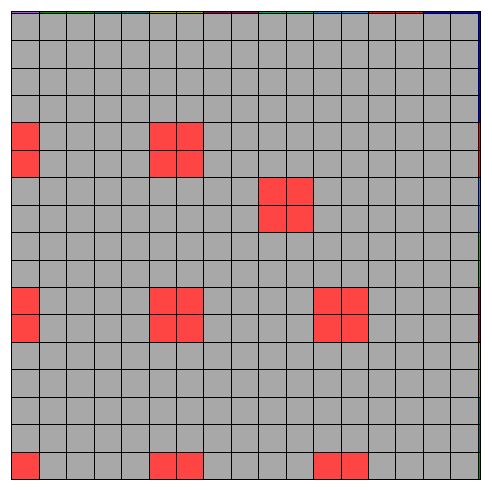
\includegraphics[width=4in]{problem3_radial_mat.png}
  \end{center}
  \caption{\textbf{Fuel assembly mesh and geometry cross section.}
    \textit{Reflecting boundaries are used on the left and lower
      boundaries to create a complete $17 \times 17$ assembly
      geometry. Gray regions are homogenized fuel and red regions are
      homogenized moderator. Each fuel pin is resolved by a $2 \times
      2$ mesh.}}
  \label{fig:problem3_radial_mat}
\end{figure}
\begin{figure}[t!]
  \begin{center}
    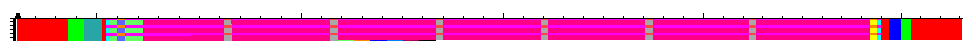
\includegraphics[width=6.0in]{problem3_axial_mat.png}
  \end{center}
  \caption{\textbf{Fuel assembly geometry cross section.} \textit{The
      geometry is subdivided along the axial direction into 50 zones
      spaced to capture material boundaries. Important details include
      spacer grids along the length of the fuel pins and reactor core
      structures on the top and bottom of the assembly. Lighter purple
      material in the center of the assembly is moderator and darker
      purple/red material is fuel.}}
  \label{fig:problem3_axial_mat}
\end{figure}
\begin{figure}[t!]
  \begin{center}
    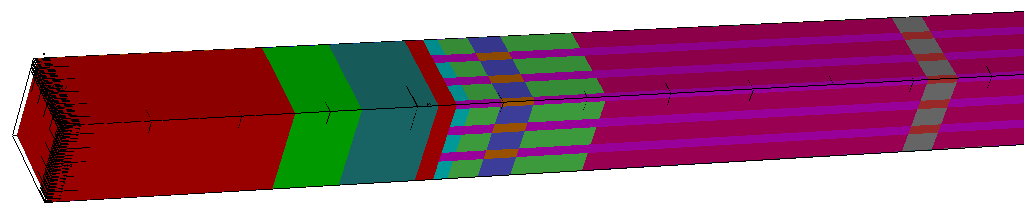
\includegraphics[width=6.0in]{problem3_end.png}
  \end{center}
  \caption{\textbf{Fuel assembly geometry end detail.}
    \textit{Reactor core structure including spacer grids and plenum
      has been included. Lighter purple material on the right of the
      figure is moderator and darker purple/red material is fuel.}}
  \label{fig:problem3_end}
\end{figure}

Significant geometric details are contained in the model including
spacer grids, fuel pins with homogenized cladding and gas gap, core
plenum, and moderator with boron. Group cross sections and other
discrete nuclear data are generated as needed by a cross-section
processing module dependent on the meshing parameters used to
discretize the geometry and single-dimension pin-cell calculations for
initial flux spectrum generation. Table~\ref{tab:problem3_parameters}
gives the primary design parameters for the fuel assembly
calculations.
\begin{table}[h!]
  \begin{center}
    \begin{tabular}{ll}\hline\hline
      \multicolumn{1}{l}{\textbf{Parameter}} & 
      \multicolumn{1}{l}{\textbf{Value}} \\
      Power Level & 0 MW \\
      Inlet Temperature & 326.85C \\
      Fuel Temperature & 600C \\
      Boron Concentration & 1300 ppm \\
      Moderator Density & 0.743 g/cc \\
      Helium Density & \sn{1.79}{-4} g/cc \\
      Zirconium Density & 6.56 g/cc \\
      Stainless Steel Density & 8.0 g/cc \\
      Inconel Density & 8.19 g/cc \\
      UO2 Density & 10.257 g/cc \\
      Fuel Pin Radius (w/o clad) & 0.4096 cm \\
      %%
      \hline\hline
    \end{tabular}
  \end{center}
  \caption{\textbf{Design parameters for the $17 \times 17$ pin fuel
      assembly criticality calculation.}}
  \label{tab:problem3_parameters}
\end{table}

To generate the multiplication factor and steady-state flux
distribution for this problem, at every eigenvalue iteration MCSA is
used to solve the resulting $SP_N$ problem using the provided fission
source. Algorithm~\ref{alg:power_iteration} presents the use of MCSA
within a power iteration strategy to find the multiplication factor.
\begin{algorithm}[h!]
  \caption{Power Iteration MCSA Scheme}
  \label{alg:power_iteration}
  \begin{algorithmic}
    \State $k_0 =$ initial guess
    \State $\mathbf{\Phi}_0 =$ initial guess
    \State $n = 0$
    \While{$|\frac{k^n - k^{n-1}}{k^n}| < \epsilon$}
    \Comment{Iterate until convergence of the eigenvalue}
    \State $\mathbf{M} \mathbf{\Phi}^{n+1} = \frac{1}{k^n} \mathbf{F} \mathbf{\Phi}^n$
    \Comment{Solve for the new flux state with MCSA}
    \State $k^{n+1} = k^n \frac{\int \mathbf{F} \mathbf{\Phi}^{n+1} d\mathbf{r}}{\int
      \mathbf{F} \mathbf{\Phi}^n d\mathbf{r}}$
    \Comment{Update the multiplication factor}
    \State $n = n+1$
    \EndWhile
  \end{algorithmic}
\end{algorithm}
Here, $\mathbf{M}$ is the transport operator generated on the
left-hand side of the $SP_N$ discretization, $\mathbf{F}$ is the
fission matrix, and $\mathbf{\Phi}$ the multigroup neutron flux. This
problem is significantly more complicated than the simple test problem
used for the previous spectral analysis. Fission has been introduced
into the set of equations and the addition of moderator into the
system will increase the amount of scattering, creating a
significantly more difficult problem manifesting itself in an
iteration matrix with a larger spectral radius. When using MCSA, the
linear operator applied to $\mathbf{\Phi}^{n+1}$ at each eigenvalue
iteration will dictate convergence and remain unchanged throughout the
computation\footnote{The operator will change if, for example, physics
  feedback through temperature or potentially burnup is
  considered. These additional physics will modify the cross sections
  used to assemble $\mathbf{M}$. The calculations presented here will
  consist of a single eigenvalue calculation with a static
  $\mathbf{M}$.} while the addition of fission to the system will only
modify the source of neutrons and the multiplication factor while not
affecting Monte Carlo transport.

%%---------------------------------------------------------------------------%%
\section{Preconditioned MCSA}

In most cases, at least a minimal amount of \textit{preconditioning}
of the linear system will be required in order to use the class of
stochastic methods described. Although these methods have no symmetry
requirements for convergence, they do require that the spectral radius
of the iteration matrix be less than one. Preconditioning serves as a
means of achieving this by altering the eigenvalue spectrum of the
iteration matrix. It is possible to use general left, right, and left/right
preconditioning with MCSA by carefully considering the underlying
Monte Carlo problem that will be solved with the Neumann-Ulam
method. We consider here the general left/right preconditioned method
as the left or right preconditioned methods can be inferred from its
formulation. 

We consider a left preconditioner $\ve{M_L}$ and a right
preconditioner $\ve{M_R}$. The left/right preconditioned linear
problem is then:
\begin{equation}
  \ve{M}_L^{-1}\ve{A}\ve{M}_R^{-1}\ve{M}_R\ve{x} = \ve{M}_L^{-1}\ve{b}\:.
  \label{eq:left_right_linear_problem}
\end{equation}
To handle the right preconditioning, the system is written with a
substitution of variables:
\begin{equation}
  \ve{M}_L^{-1}\ve{A}\ve{M}_R^{-1}\ve{u} = \ve{M}_L^{-1}\ve{b}\:,
  \label{eq:left_right_subs_problem}
\end{equation}
with
\begin{equation}
  \ve{x} = \ve{M}_R^{-1}\ve{u}\:.
  \label{eq:left_right_recover}
\end{equation}
To apply such a method to MCSA, we solve for the substituted variable
$\ve{u}$ during the iteration sequence:
\begin{subequations}
  \begin{gather}
    \ve{u}^{k+1/2} = \ve{u}^k + \ve{r}^k\:,\\
    \ve{r}^{k+1/2} = \ve{M}_L^{-1}(\ve{b}-\ve{A}\ve{M}_R^{-1}\ve{u}^{k+1/2})\:,\\ 
    \ve{M}_L^{-1}\ve{A}\ve{M}_R^{-1}\delta\ve{u}^{k+1/2} = \ve{r}^{k+1/2}\:,\\ 
    \ve{u}^{k+1} = \ve{u}^{k+1/2} + \delta \ve{u}^{k+1/2}\:,\\
    \ve{r}^{k+1} = \ve{M}_L^{-1}(\ve{b}-\ve{A}\ve{M}_R^{-1}\ve{u}^{k+1})\:,
  \end{gather}
  \label{eq:left_right_mcsa}
\end{subequations}
and then recover the original solution vector with
Eq~(\ref{eq:left_right_recover}). For the Monte Carlo problem, we
isolate the generation of the correction:
\begin{equation}
  \ve{M}_L^{-1}\ve{A}\ve{M}_R^{-1}\delta\ve{u}^{k+1/2} = \ve{r}^{k+1/2}\:,
  \label{eq:left_right_correction}
\end{equation}
and note that the preconditioned residual of the substituted variable
is now serving as the source and the new iteration matrix is:
\begin{equation}
  \ve{H} = \ve{I} - \ve{M}_L^{-1}\ve{A}\ve{M}_R^{-1}\:.
  \label{eq:left_right_iteration_matrix}
\end{equation}
As we require $(i,j)$ element-wise access to the iteration matrix in
order to construct probabilities and weights for the Monte Carlo
procedure from the Neumann-Ulam decomposition, the \textit{composite
  operator}, $\ve{M}_L^{-1}\ve{A}\ve{M}_R^{-1}$, must be formed via
matrix-matrix multiplication. 

Several possible shortcomings of this preconditioning approach are
readily observed. First, the matrix-matrix multiplication operation
for sparse, parallel distributed matrices is significantly more
expensive than a matrix-vector multiplication operation. Second, each
preconditioner must be explicitly inverted, an operation in itself
that may be expensive and which prohibits the use of any
preconditioners which provide no mechanism to extract their
inverse. Third, for many modern preconditioning methods, this
inversion may yield dense matrices, destroying sparsity and further
impeding the performance of a matrix-matrix multiplication
operation. It is also interesting to note that the Monte Carlo problem
in the general left/right preconditioned scheme given by
Eq~(\ref{eq:left_right_correction}) is not fully left/right
preconditioned (meaning that we do not recover $\ve{x}$), but instead
part of a sequence for finding the substituted variable $\ve{u}$. We
do, however, gain the benefits of this general preconditioning by
building the iteration matrix in
Eq~(\ref{eq:left_right_iteration_matrix}) from the fully
preconditioned linear operator. In addition, for MCSA to apply to
increasingly difficult problems, more advanced preconditioning
techniques that require the generation of the composite operator may
be necessary for convergence.

\subsection{Preliminary Jacobi Preconditioned Calculations}
\label{subsec:jacobi_prec_assembly_calc}
Based on the success of block Jacobi preconditioning with the test
problem used for the spectral radius parameter study, we use it first
to solve the $17 \times 17$ fuel assembly problem. A single energy
group problem was first solved with $SP_1$ discretization, effectively
giving the one-speed neutron diffusion system for the fuel assembly
resulting in 20,088 degrees of freedom in the
problem. Figure~\ref{fig:block_jacobi_res_mcsa} gives the residual
infinity norm as a function of iteration for the MCSA linear solve in
the first eigenvalue iteration using 25,000 stochastic histories at
every iteration for the adjoint Neumann-Ulam solve.
\begin{figure}[t!]
  \begin{center}
    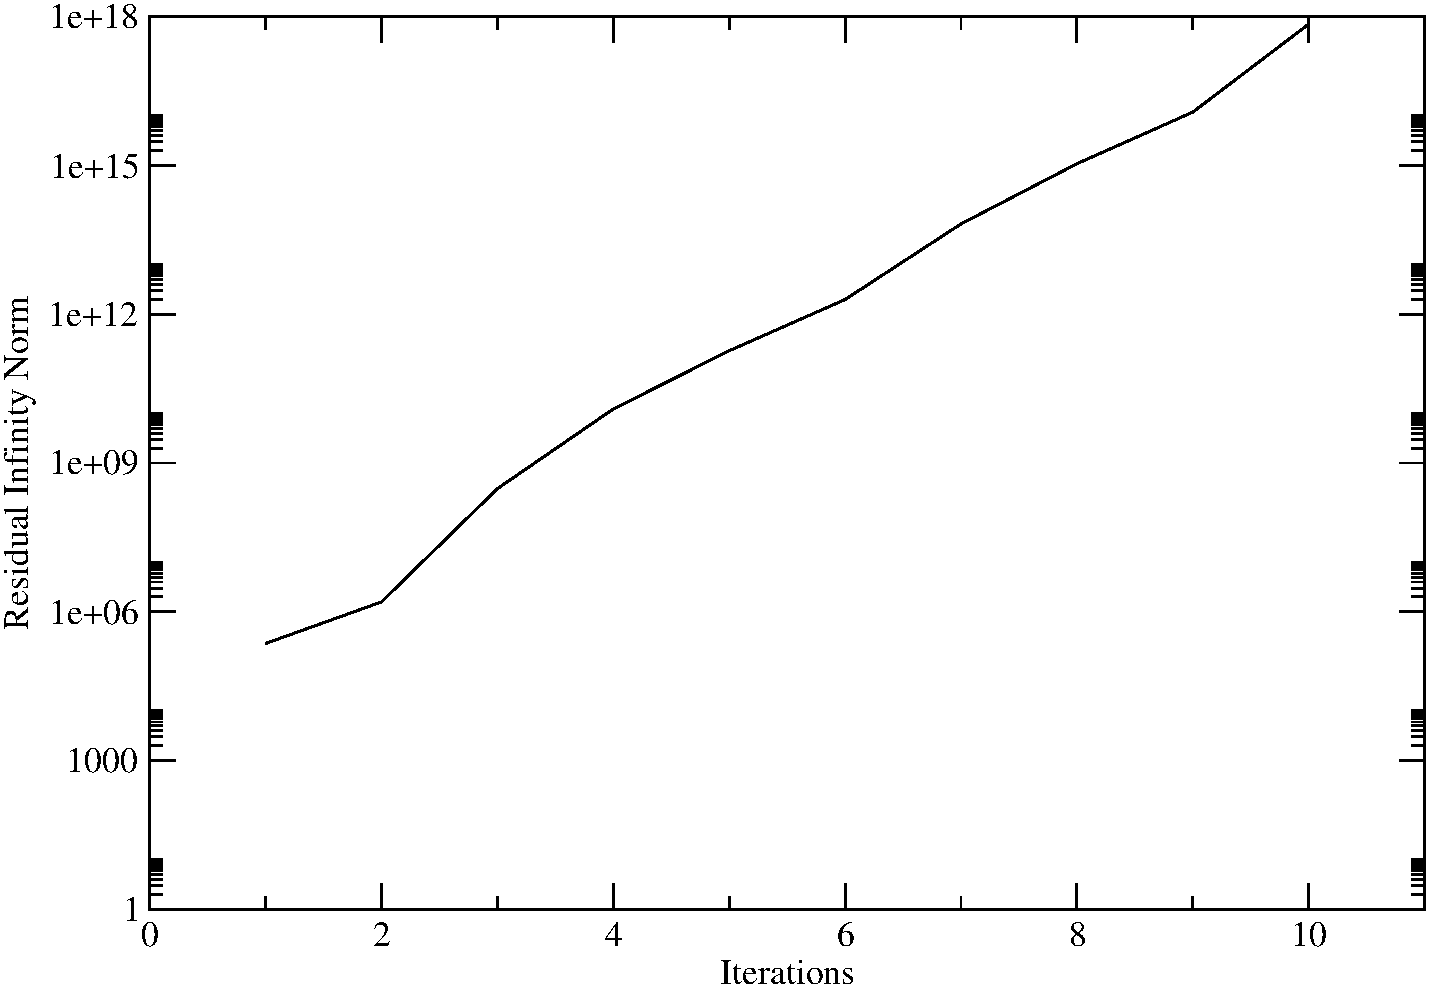
\includegraphics[width=5in]{block_jacobi_res.pdf}
  \end{center}
  \caption{\textbf{Residual infinity norm vs. iteration for the block
      Jacobi preconditioned MCSA solve during the first eigenvalue
      iteration of the 1-group $17 \times 17$ fuel assembly problem.}
    \textit{Convergence was not achieved with the block Jacobi
      preconditioned method.}}
  \label{fig:block_jacobi_res_mcsa}
\end{figure}
Convergence was not achieved as noted by the rapid rise in the
residual over a few iterations. Based on the spectral radius
computations performed, these results are not in line with
expectations for this problem. Additional computations performed with
\sn{1}{6} histories per iteration exhibited the same divergent
behavior at a significant computational cost and compute time. Even if
the problem may be ill-conditioned, we do expect convergence of
MCSA. To investigate further, a block Jacobi preconditioned Richardson
iteration was used to solve the same
problem. Figure~\ref{fig:block_jacobi_res_richardson} gives the
residual infinity norm as a function of iteration for the Richardson
linear solve in the first eigenvalue iteration.
\begin{figure}[t!]
  \begin{center}
    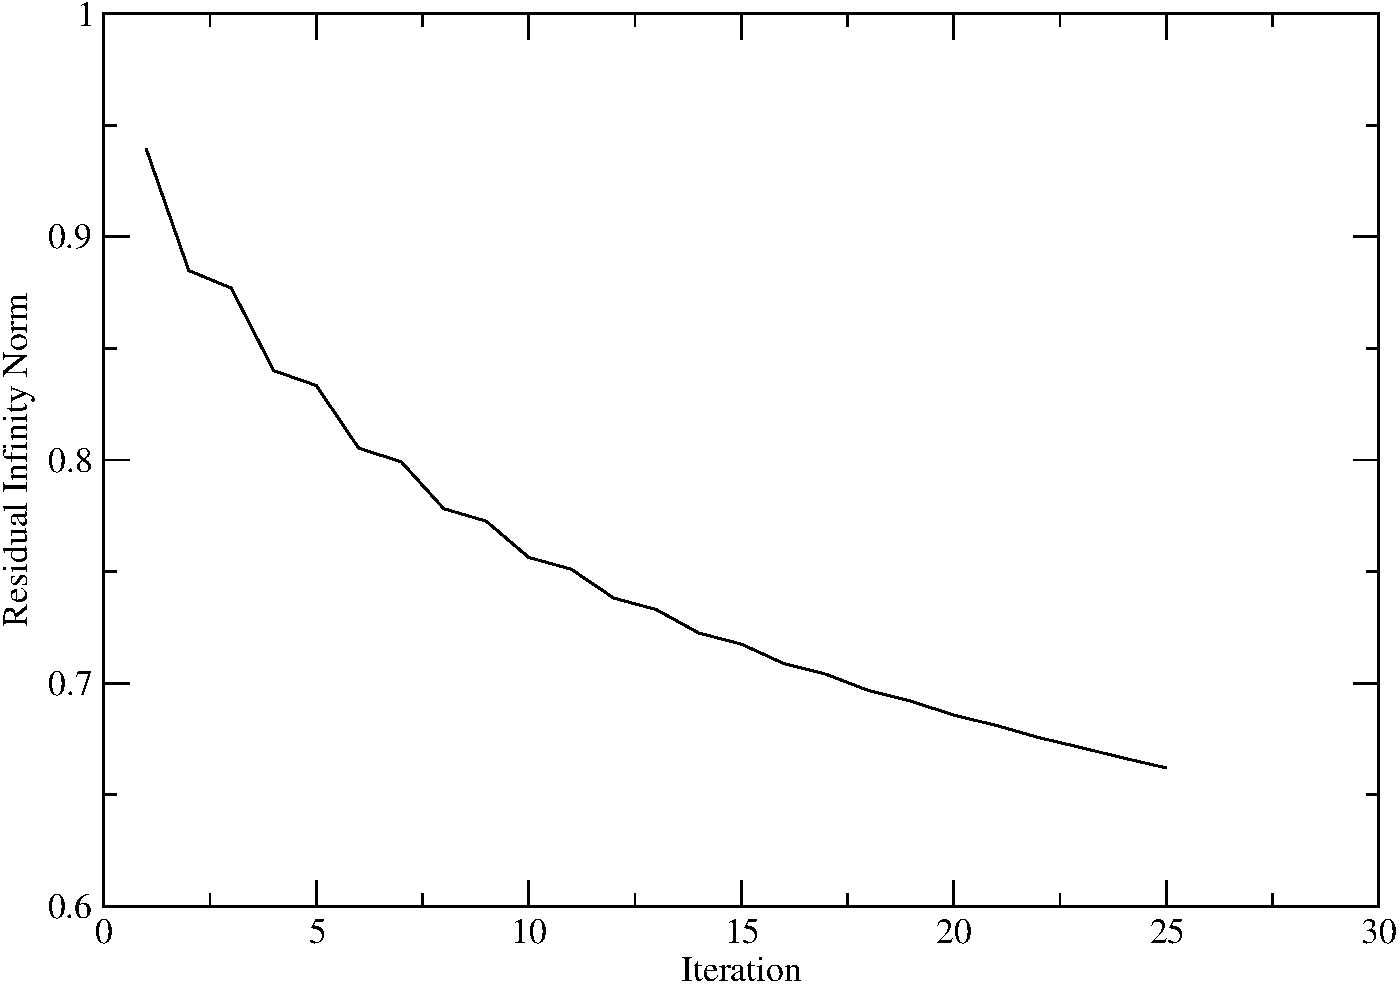
\includegraphics[width=5in]{block_jacobi_rich_res.pdf}
  \end{center}
  \caption{\textbf{Residual infinity norm vs. iteration for the block
      Jacobi preconditioned Richardson solve during the first
      eigenvalue iteration of the 1-group $17 \times 17$ fuel assembly
      problem.} \textit{A spectral radius near 1 was observed for the
      iteration matrix.}}
  \label{fig:block_jacobi_res_richardson}
\end{figure}
Poor converge is observed for the Richardson iteration, however,
convergence is achieved meaning that the preliminary eigenvalue
criteria needed to satisfy MCSA convergence has also been met. The
number of iterations required for the Richardson iteration to converge
will give an approximation for the spectral radius via
Eq~(\ref{eq:linear_k_iter_norm3}). With 7291 iterations required to
converge to a tolerance of $\sn{1}{-6}$, $\rho(\mathbf{H}) \approx
0.998$, nearing the limits of MCSA applicability and well beyond the
spectral radii generated in the initial spectral analysis.

Based on these results, it then appears that even if the simple
criteria of a spectral radius of less than one is met and the
Richardson iteration will converge with the same preconditioning, MCSA
still may not converge. We then expect the issue to reside with the
Neumann-Ulam solve providing the correction as the Richardson
iteration is known to provide the correct result. Furthermore, the
fact that the spectral radius is less than one means that the
stochastic histories in the block Jacobi preconditioned Neumann-Ulam
method are eventually being terminated by the weight cutoff as no
artificial absorption was used for these preliminary
calculations. Based on this, the correction being generated by the
Neumann-Ulam solve is the component of MCSA causing a divergent
solution.

\subsection{MCSA Breakdown}
\label{subsec:mcsa_break_down}
For the fuel assembly problem, the initial block Jacobi
preconditioned\footnote{For 1-group $SP_1$ problems the block size is
  1, giving a point Jacobi preconditioner.}  calculations used a
one-speed $SP_1$ discretization, effectively giving a diffusion
system. To study the breakdown of MCSA at iteration matrix spectral
radii near one, we will use the simpler homogeneous 2-dimensional
one-speed neutron diffusion system presented in
Appendix~\ref{chap:diffusion_problem} to isolate this behavior. In
this system, we can vary the cross sections while maintaining a fixed
grid in order to achieve varying spectral radii. For these studies, we
neglect fission as MCSA behavior is dictated by the transport operator
$\mathbf{M}$ in an eigenvalue scheme with the fission matrix used to
generate a fixed source.

For each solver and estimator combination, the spectral radius of the
iteration matrix generated by the diffusion problem was varied by
changing the absorption cross section from 0.25 to 100 while fixing
the grid size at $100 \times 100$ with $h = 0.1$ and a fixed
scattering cross section of unity. For each parameter variation, a
minimum of one stochastic history per degree of freedom (DOF) in the
problem was used to compute the Monte Carlo correction. If the solver
could not converge in less than 100 iterations, the number of
histories was increased by increments of 5,000 until convergence was
achieved in less than 100 iterations. The number of iterations
required to converge MCSA and the time to converge was recorded as a
means to capture the breakdown.

Figure~\ref{fig:breakdown_iterations} gives the number of iterations
required to converge for the chosen number of histories per iteration
given by Figure~\ref{fig:breakdown_histories} using the adjoint solver
with the collision and expected value estimators and the forward
solver with the collision estimator. For spectral radii less than
0.97, all MCSA problems converged with 1 history per DOF (10,000 for
this problem) with the number of iterations required to converge
increasing as a function of spectral radius. Near a spectral radius of
0.97, the number of histories required to converge MCSA in less than
100 iterations takes a dramatic rise that exhibits neither exponential
nor power law behavior. As the spectral radius approaches 1, the
number of histories required becomes significant and effectively
impractical to compute. Even with this simple diffusion problem, the
behavior is consistent with that observed for the fuel assembly
problem with $SP_1$ discretization. In that case, we estimated a
spectral radius of $\approx 0.998$, larger than any of the spectral
radii that could be computed within even 90 minutes of compute time
for this simple two dimensional problem. For that problem, even
1,000,000 histories ($\approx 50$ per DOF) was not enough to provide
convergence. Even if single solve times of an hour can be tolerated,
dozens of solves are typically required to compute the multiplication
factor and flux spectrum within the $SP_N$ eigenvalue scheme for more
difficult problems like the fuel assembly, making the method unusable.
\begin{figure}[t!]
  \begin{center}
    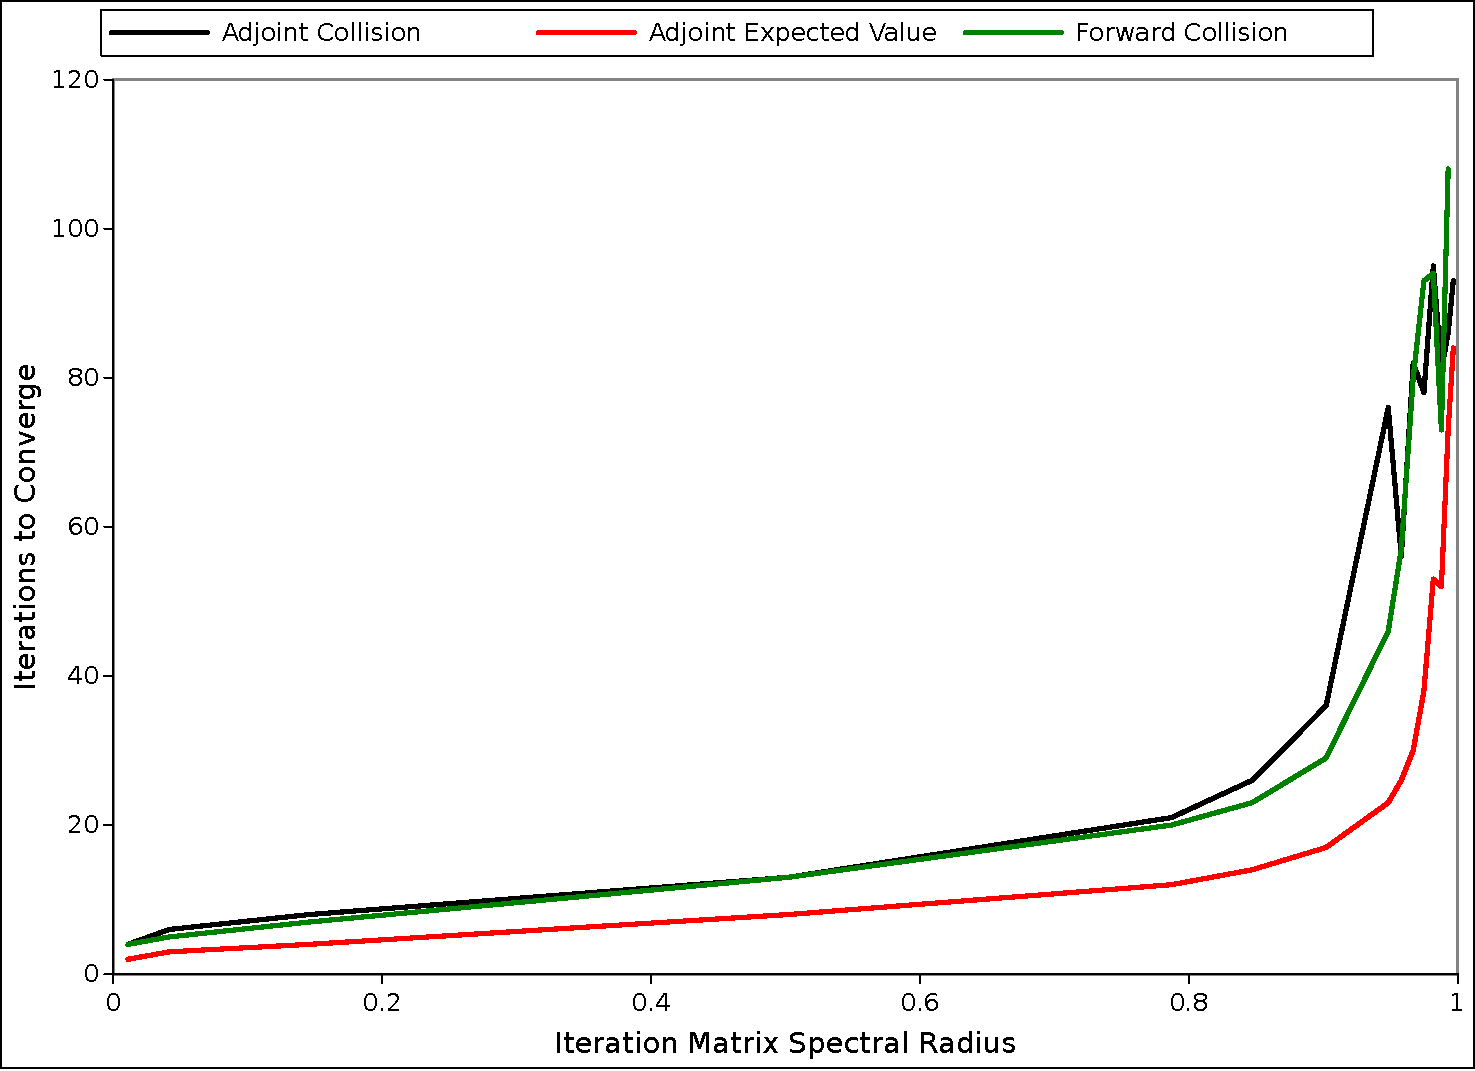
\includegraphics[width=4.25in]{breakdown_iterations.pdf}
  \end{center}
  \caption{\textbf{Iterations required to converge as a function of
      spectral radius for the neutron diffusion problem.} \textit{The
      number of histories was increased to achieve convergence in less
      than 100 iterations. At least 10,000 histories were used for
      each calculation.}}
  \label{fig:breakdown_iterations}
\end{figure}
\begin{figure}[t!]
  \begin{center}
    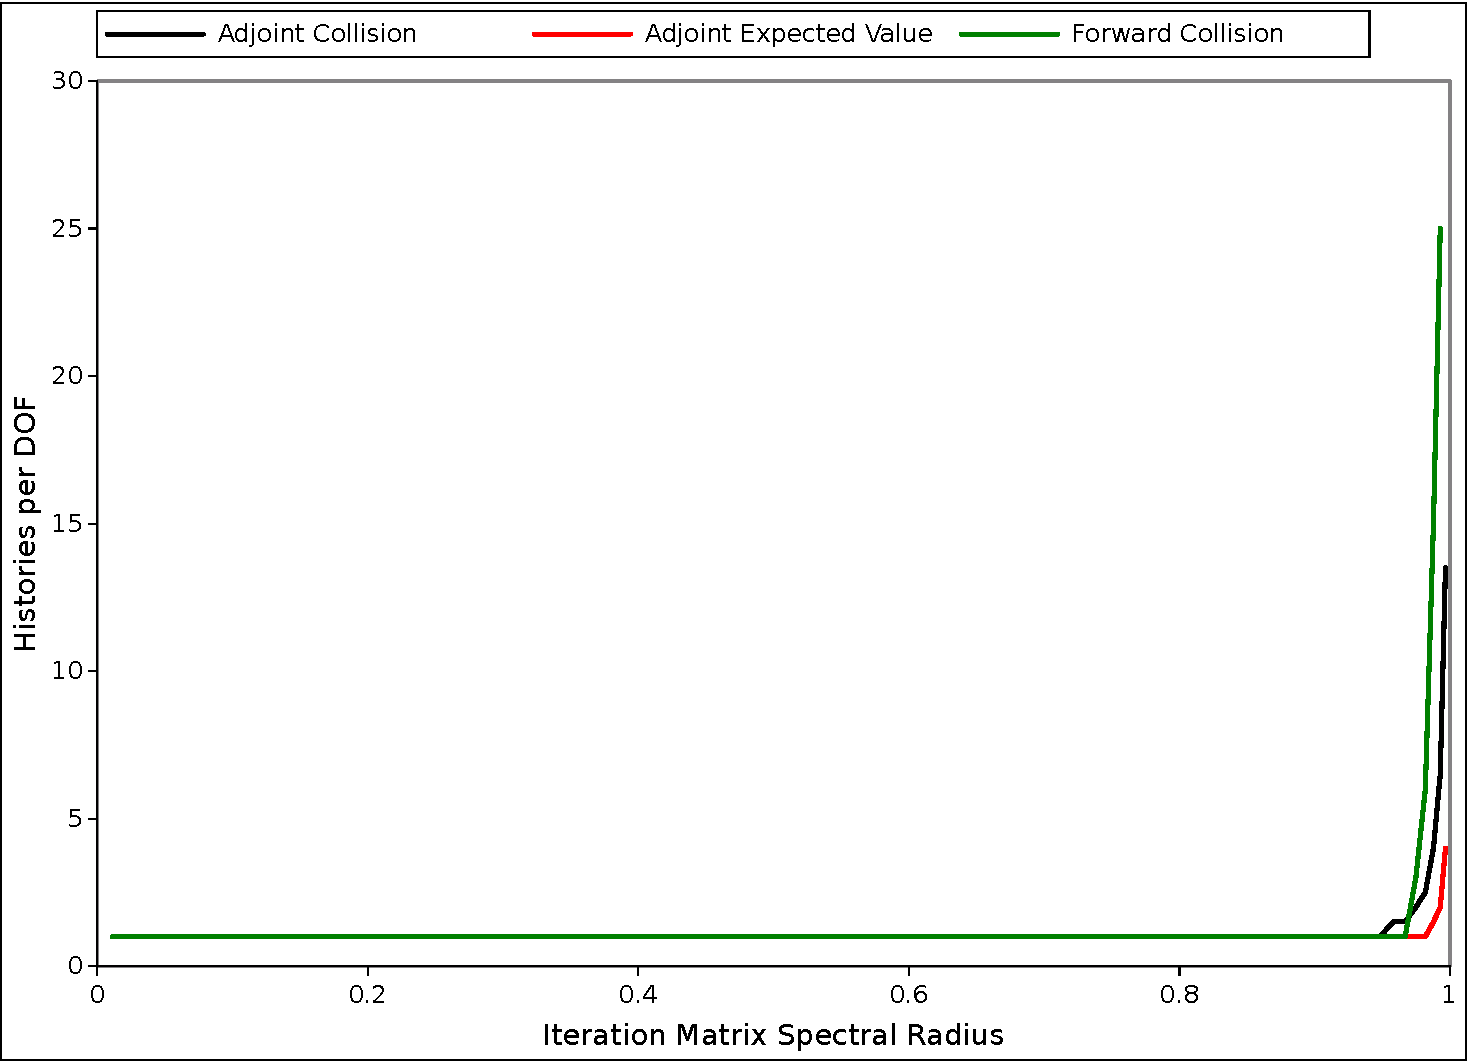
\includegraphics[width=4.25in]{breakdown_histories.pdf}
  \end{center}
  \caption{\textbf{Histories per DOF required to converge as a
      function of spectral radius for the neutron diffusion problem.}
    \textit{The number of histories was increased to achieve
      convergence in less than 100 iterations. At least 10,000
      histories were used for each calculation with 10,000 DOFs in the
      problem.}}
  \label{fig:breakdown_histories}
\end{figure}

In addition to the significantly larger number of histories required
to achieve convergence for ill-conditioned problems another penalty is
paid due to histories that take longer to
compute. Figure~\ref{fig:breakdown_time} gives the CPU time in seconds
required to compute a single random walk averaged over the entire set
of histories run in the calculation over all iterations. As the
spectral radius increases (correlating to a higher ratio of scattering
in the system) the random walk lengths increase, using more CPU time
to finish the computation. Compared to spectral radii of 0.5, larger
spectral radii over 0.97 have histories that require two orders of
magnitude more computation time. This significant increase in
computation time per history coupled with the significant increase in
the number of histories required to converge is evidence that for
problems with spectral radii above $\approx 0.97$, using MCSA to solve
any problems of interest is entirely ineffective and not practical. We
therefore require a more expansive set of preconditioning techniques
to move the eigenvalue spectrum of the $SP_N$ problem into a regime in
which MCSA is more applicable and in which performance is improved.
\begin{figure}[t!]
  \begin{center}
    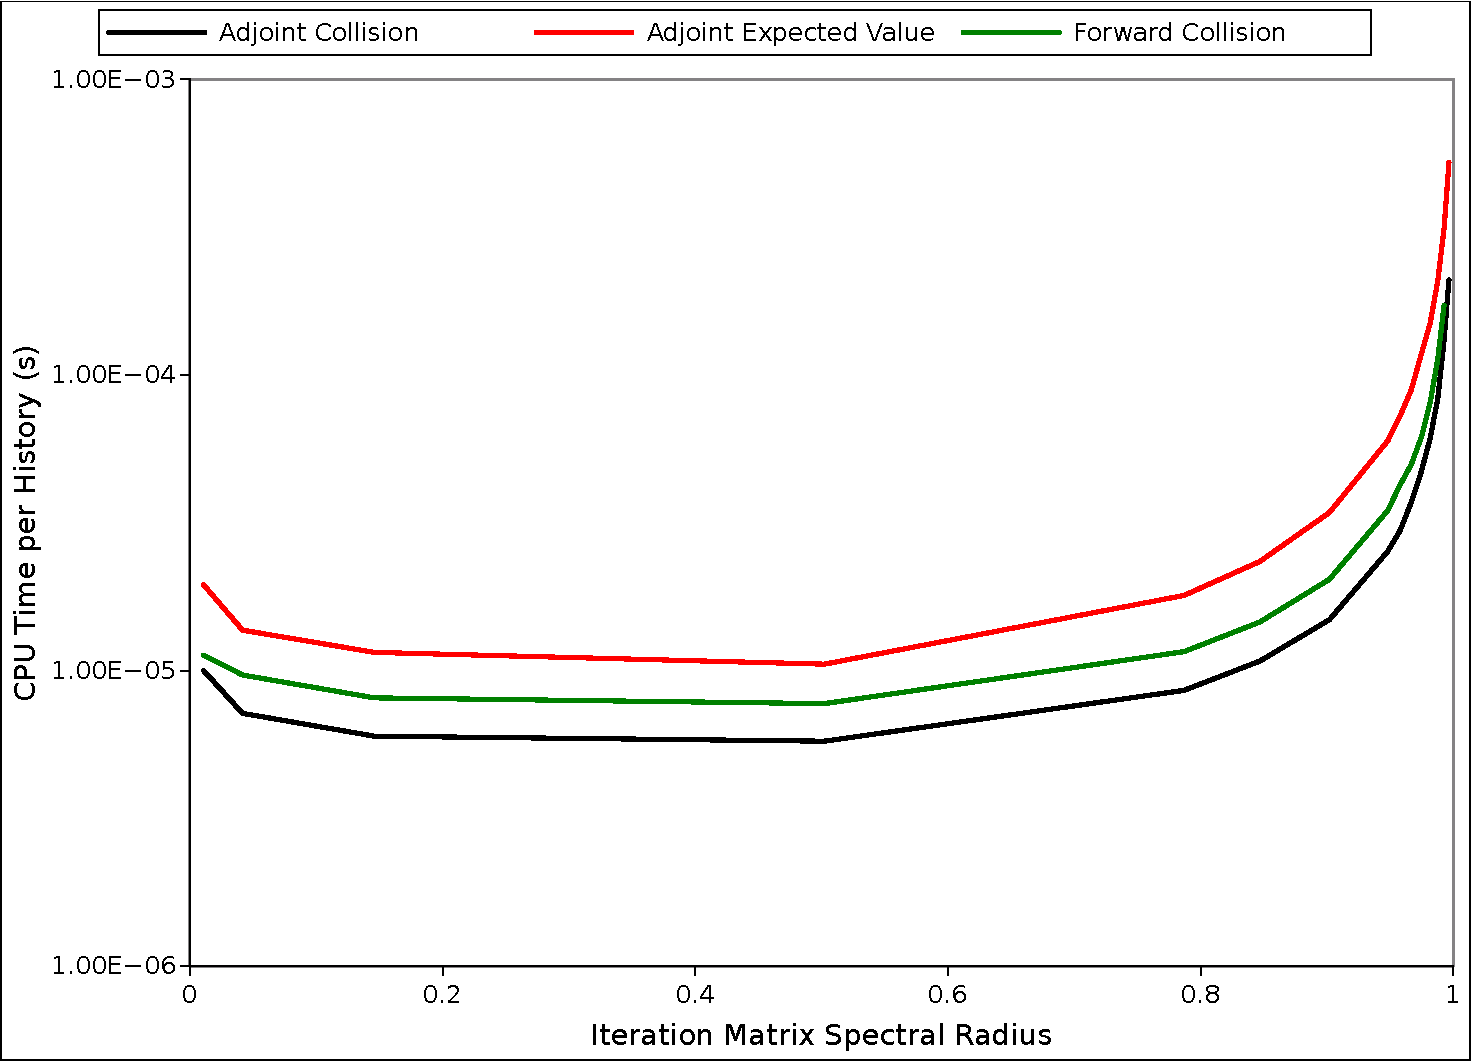
\includegraphics[width=4.25in]{breakdown_time.pdf}
  \end{center}
  \caption{\textbf{CPU time per history as a function of spectral
      radius for the neutron diffusion problem.} \textit{As the
      spectral radius grows, so do the length of the random
      walks. Longer random walks require more CPU time to compute.}}
  \label{fig:breakdown_time}
\end{figure}

\subsection{Algebraic Preconditioning Strategies}
\label{subsec:spn_advanced_preconditioning}
For the fuel assembly criticality problem presented in the previous
section, the spectral radius was near one using Jacobi preconditioning
and in a regime in which MCSA breakdown is observed. In this regime
the number of stochastic histories required to converge MCSA increases
rapidly and the resulting poor performance is compounded by those
histories being increasingly expensive to compute. To overcome this
difficulty, advanced preconditioning strategies for the $SP_N$ problem
are required beyond simple Jacobi methods that can reduce the spectral
radius into a region of better MCSA performance. Several modern
algebraic preconditioning strategies will be presented here and used
within the explicit preconditioning framework given by
Eq~(\ref{eq:left_right_mcsa}). Data showing their effects on MCSA
solutions of the fuel assembly criticality problem will be presented.

\subsection{ILUT Preconditioning}
\label{subsec:spn_ilut_preconditioning}
Incomplete lower-upper (ILU) factorizations of the linear operator can
be used a simple mechanism to form an approximate inverse of a
preconditioner. To build the factorization, the sparse upper and lower
triangular factors, $\mathbf{L}$ and $\mathbf{U}$, are computed such
that the residual matrix formed by the factorization
\cite{saad_iterative_2003}:
\begin{equation}
  \mathbf{R} = \mathbf{L} \mathbf{U} - \mathbf{A} \:,
  \label{eq:ilu_residual_matrix}
\end{equation}
has a specified sparsity pattern and element magnitude. When a
magnitude threshold is used, elements generated in the factors below
that magnitude are dropped, resulting in ILU threshold (ILUT)
preconditioning. The sparsity pattern in this case is determined from
the input matrix to be preconditioned and the number of elements
maintained in the factor is specified by a fill level parameter. A
fill level of 1 will generate the same number of elements as the
sparsity pattern of the input matrix while a fill level of 2 will
contain twice as many elements in the factorization, resulting in a
better representation of the true LU factorization. The inverse of the
lower and upper triangular factors may then be easily inverted by
means of simple elimination to produce the preconditioner. For MCSA,
$\mathbf{L}^{-1}$ will be used on the left and $\mathbf{U}^{-1}$ on
the right to precondition the system.

For modern subspace methods, only the action to the preconditioner on
a vector is required for efficient implementations and therefore a
triangular solve can be used for this purpose. For the explicit
preconditioning scheme presented in Eq~(\ref{eq:left_right_mcsa}), the
fully inverted operator must be generated in order to build the set of
probabilities and weights required for Monte Carlo
sampling. Therefore, for a linear system of size $N$, $N$ triangular
solves will be required in order to extract the inverse matrices from
production ILU implementations. In addition, parallel implementations
typically generate lower and upper factors that are only triangular
locally, providing an easily parallelizable mechanism to generate the
action of the preconditioner inverse. A consequence of this choice for
parallel scalability is a degradation of the preconditioning quality
as the size of the parallel system is increased. For serial
computations, the triangular factorization is potentially exact
depending on the parameters chosen while at thousands of parallel
tasks, the global triangular factors differ significantly from the true
factorization. As a result, more iterations are required at higher
levels of parallelism to converge the system and will ultimately
degrade overall scalability of the system with respect to total wall
time to converge.

MCSA preconditioned with ILUT was used to solve the fuel assembly
problem presented in the previous section for a 1-group $SP_1$
discretization. Unlike the Jacobi preconditioned strategy, convergence
was achieved with ILUT preconditioning. To study convergence
sensitivity to ILUT parameters, the fill level and drop tolerance were
parametrically varied with the number of iterations to converge an
eigenvalue iteration for the fuel assembly problem recorded along with
the maximum number of non-zero entries observed in all matrix rows for
the left/right preconditioned composite linear operator. To provide
some sparsity to the factorization, the ILUT drop tolerance was used
to drop elements in the extracted inverse triangular factors. For each
calculation, the number of iterations required to converge reported
was for a single eigenvalue iteration with \sn{3}{4} histories at each
MCSA iteration to compute the Monte Carlo correction using the adjoint
collision estimator. All ILUT calculations reported here were
performed on a single CPU and therefore this data does not take into
account the aforementioned effects of parallel decomposition on the
quality of the ILUT preconditioning.

Figure~\ref{fig:ilut_iterations} gives the number of iterations to
converge the fixed source problem to a tolerance of \sn{1}{8}. As
expected, the higher the fill level chosen for the ILUT factorization,
the fewer iterations are required to converge the problem (only 9 MCSA
iterations were required to converge the problem for the fill level of
3 and drop tolerance of \sn{1}{-5} case). For higher levels of fill,
the iterations needed to converge were not as sensitive, signaling
that a larger drop tolerance can perhaps be used without a significant
degradation in iterative performance. At smaller fill levels, the
sensitivity to the ILUT drop tolerance is more significant. For all
fill levels used, convergence was not achieved for the fuel assembly
problem with a drop tolerance larger than \sn{1}{-3}.
\begin{figure}[t!]
  \begin{center}
    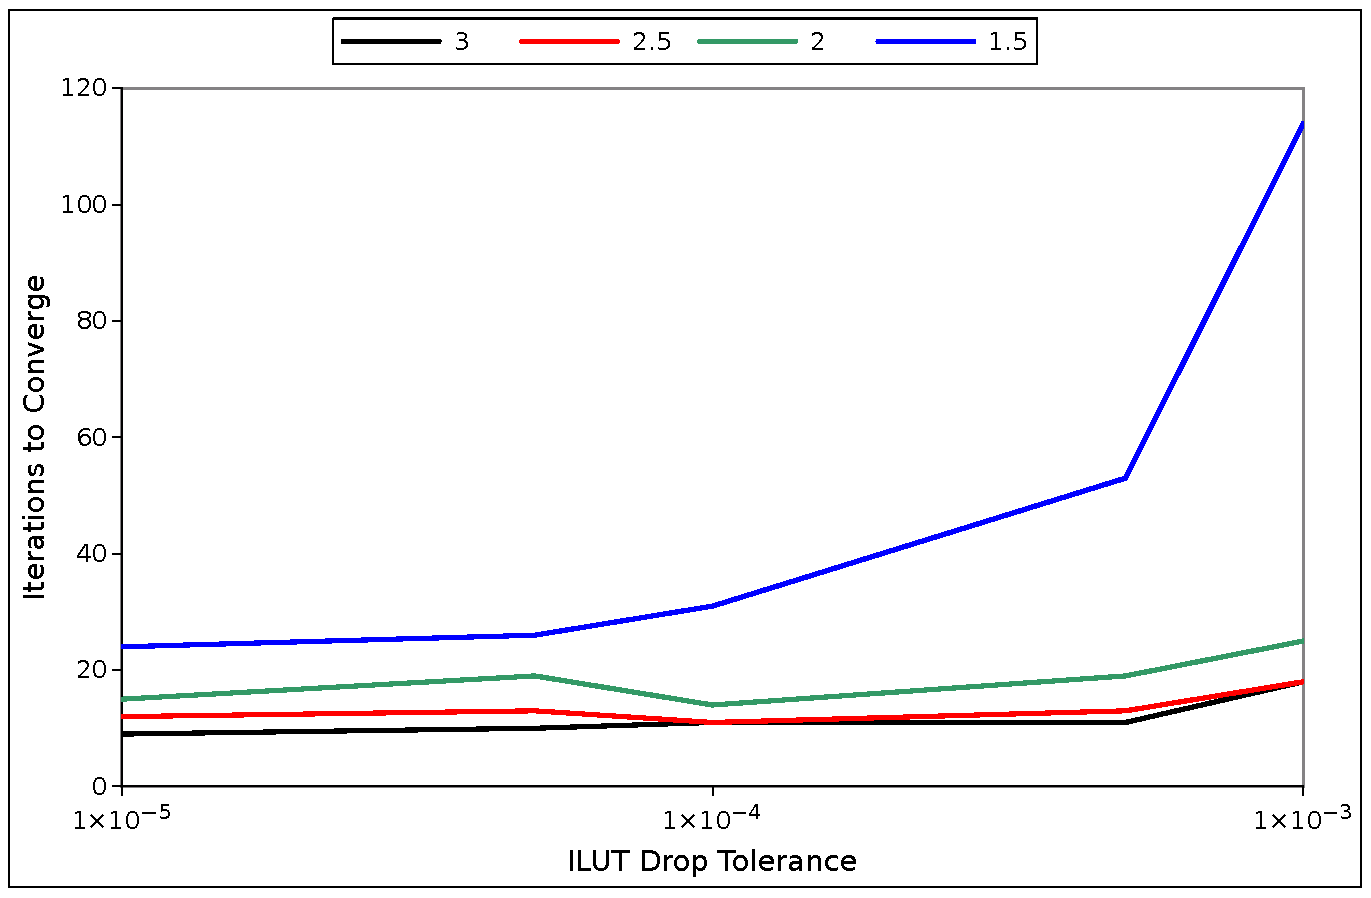
\includegraphics[width=4.25in]{ilut_iterations.pdf}
  \end{center}
  \caption{\textbf{Number of MCSA iterations required to converge an
      eigenvalue iteration for the fuel assembly problem with ILUT
      preconditioning as a function of ILUT drop tolerance.}
    \textit{Each colored curve represents the iteration behavior for a
      different ILUT fill level. Fill levels of 1.5, 2.0, 2.5, and 3.0
      were used.}}
  \label{fig:ilut_iterations}
\end{figure}

Unfortunately, gaining convergence (and excellent iterative
performance) with MCSA for the $SP_N$ fuel assembly problem comes at
an immediate cost. Figure~\ref{fig:ilut_size} gives the maximum number
of non-zero entries in the composite linear operator generated by
preconditioning as a function ILUT drop tolerance for varying values
of fill level. For the 1-group $SP_1$ discretization, the original
linear operator will contain only a maximum of 7 non-zero entries per
row in the system. As observed in Figure~\ref{fig:ilut_size},
performing the explicit preconditioning yields composite linear
operators with $O(1,000)$ elements in a row for all combinations of
fill level and drop tolerance, over 10\% of the total row size for
this particular problem. This large number of row entries, observed
for a significant fraction of rows in the system, creates several
problems. First, sparsity is completely destroyed with each state in
the system now coupled to over 10\% of the total states in the system
through the composite iteration matrix. This means that Monte Carlo
sampling tables will be large, requiring significant memory to store
them and a substantial overhead in the sampling procedure during
transport. Second, the matrix-matrix multiply operations required to
build the composite operator see significant performance losses due to
the amount of data that must be handled. In parallel, losing sparsity
severely inhibits performance where now parallel operations require
communications among orders of magnitude more processors for
nearest-neighbor type algorithms.
\begin{figure}[t!]
  \begin{center}
    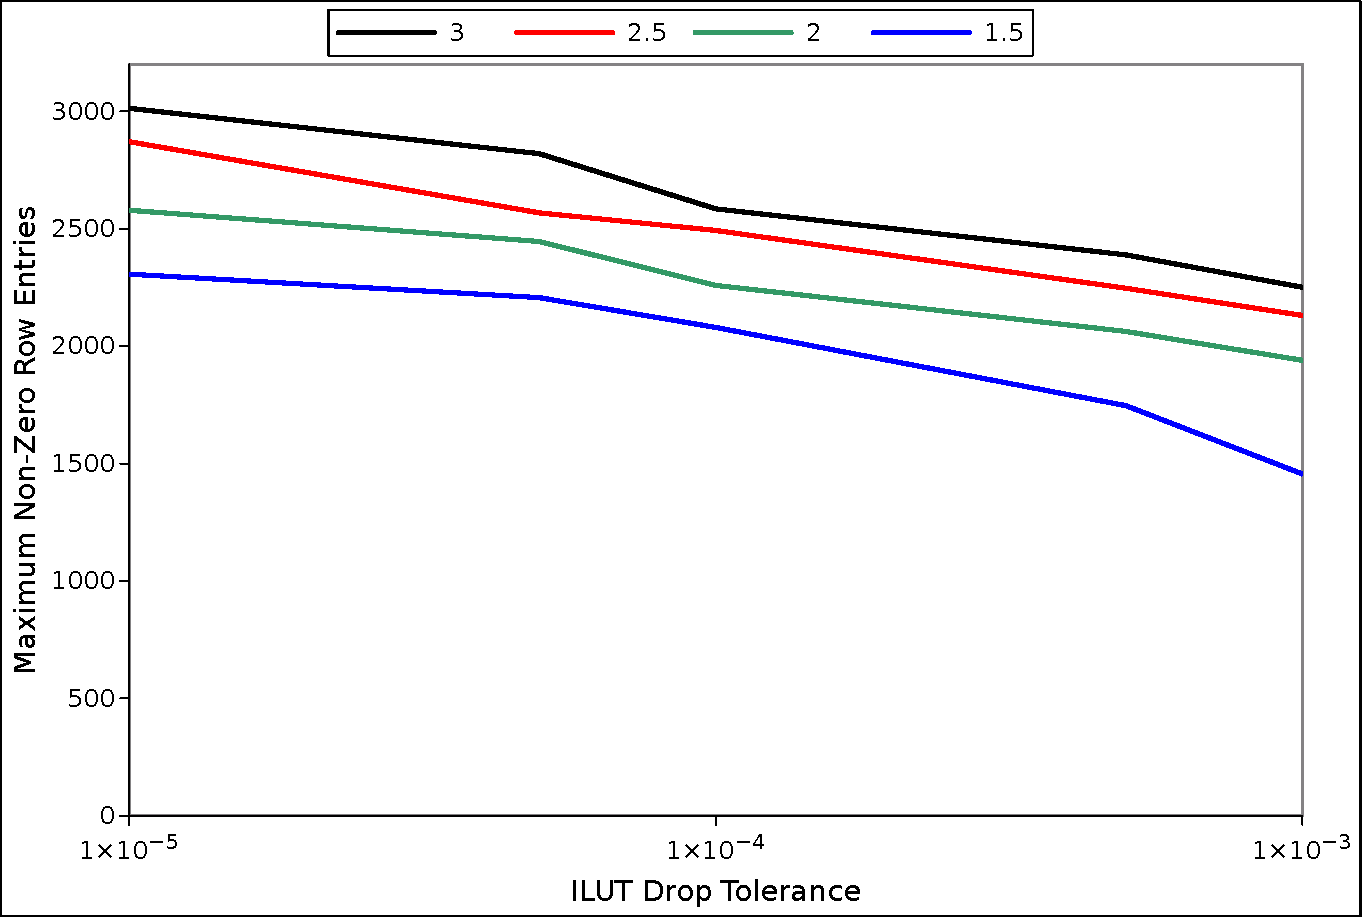
\includegraphics[width=4.25in]{ilut_size.pdf}
  \end{center}
  \caption{\textbf{Maximum number of non-zero entries observed for all
      rows in the composite linear operator for the fuel assembly
      problem with ILUT preconditioning given as a function of ILUT
      drop tolerance.} \textit{Each colored curve represents the row
      size for a different ILUT fill level. Fill levels of 1.5, 2.0,
      2.5, and 3.0 were used.}}
  \label{fig:ilut_size}
\end{figure}

As a means to assess the quality of the preconditioning, a simple
metric is developed to address these concerns and allow comparison to
future developments. For our studies, our core performance metric will
be iterative performance with the minimum number of MCSA iterations
required to converge the problem desired. For Monte Carlo
calculations, this improved performance is balanced by the creation of
a dense composite system and we seek to reduce the number of non-zero
entries to a minimum value in order to lower the amount of coupling
among states in the system and reduce the amount of memory used
along with the potential latency overhead. Given these two objectives,
the following metric is proposed:
\begin{equation}
  \text{Quality Metric} = (\text{\# iterations}) \times (\text{maximum
    \# of non-zero values})\:,
\end{equation}
where the highest quality preconditioning is one that minimizes this
metric. For the ILUT preconditioned data provided,
Figure~\ref{fig:ilut_quality} provides the computed metric as a
function of ILUT drop tolerance for each fill level used. In general,
the metric is similar to the data observed for the number of
iterations required to converge as the non-zero row entries changed by
a smaller fraction over drop tolerances tested.
\begin{figure}[t!]
  \begin{center}
    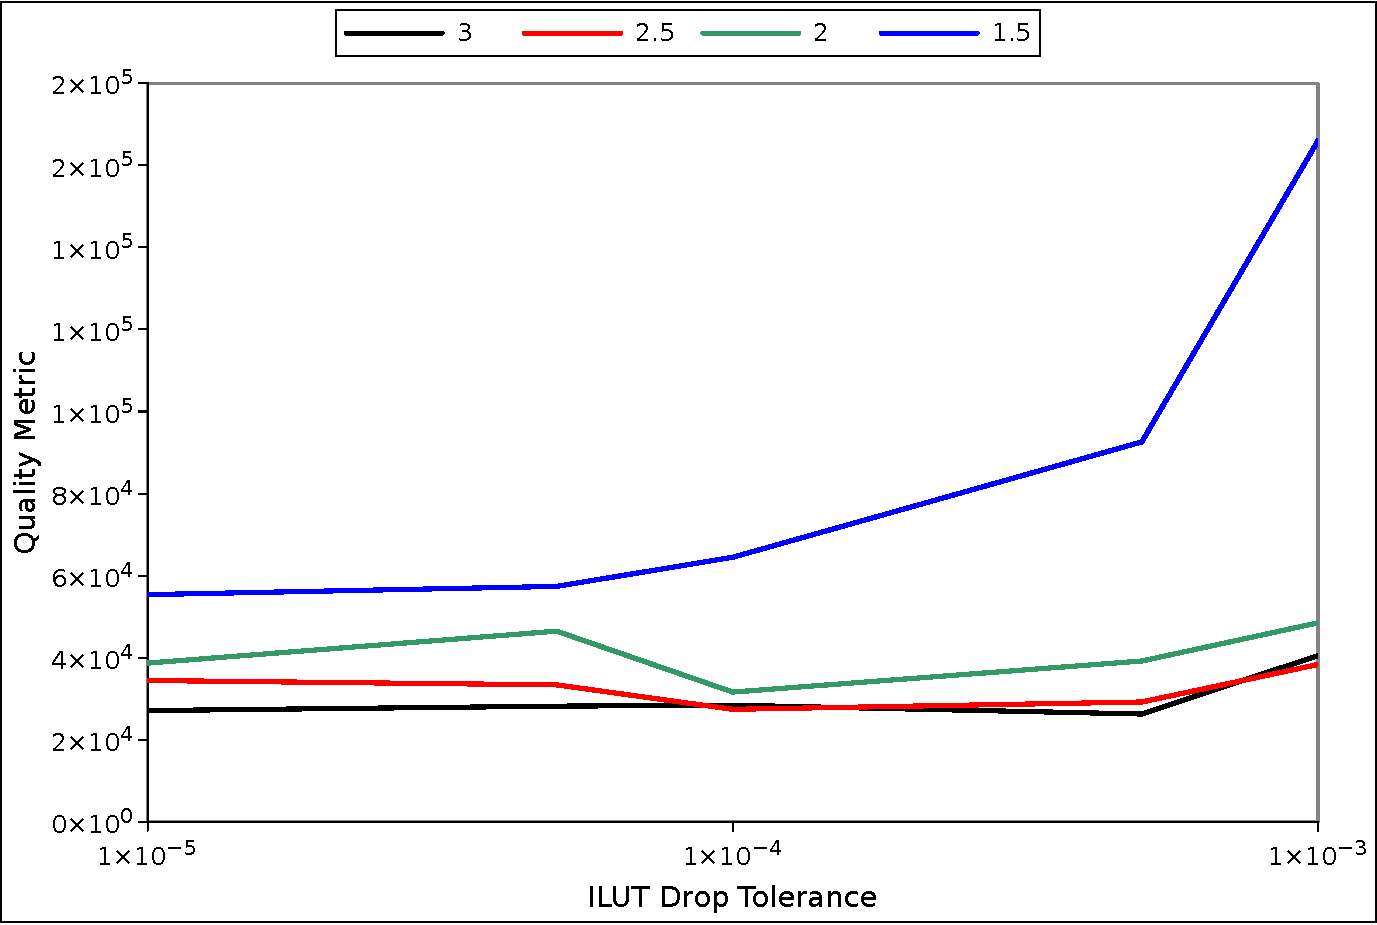
\includegraphics[width=4.25in]{ilut_quality.pdf}
  \end{center}
  \caption{\textbf{ILUT preconditioning quality metric for the fuel
      assembly problem given as a function of ILUT drop tolerance.}
    \textit{Each colored curve represents the quality metric behavior
      for a different ILUT fill level. Fill levels of 1.5, 2.0, 2.5,
      and 3.0 were used.}}
  \label{fig:ilut_quality}
\end{figure}

It should be noted here that although only the behavior of the linear
solve during a single eigenvalue iteration is reported, the behavior
of the linear solver was observed to be consistent throughout the
eigenvalue iterations (25 total eigenvalue iterations were required to
converge the 1-group $SP_1$ problem). We expect this as the linear
operator (which is unchanging in the fuel assembly criticality
problem) dictates the convergence of MCSA. At each iteration the
fission source provided to the linear problem is changing, however, we
expect the same convergence behavior for all source vectors
$\mathbf{b} \in \mathbb{R}^{N}$ where $||\mathbf{b}||_1 \neq 0$.

\subsection{Applying the Reduced Domain Approximation}
\label{subsec:spn_prec_rda}
For each preconditioning technique presented convergence was achieved
for the single fuel assembly problem. However, a primary concern is
the number of non-zero states in each row of the system generated by
the explicit preconditioning strategy. In many cases, orders of
magnitude more matrix elements were generated resulting in poor
scalability for domain decomposed algorithms and overall performance
issues for Monte Carlo. As outlined in
\S~\ref{subsec:reduced_domain_approximation}, the reduced domain
approximation may be used as a mechanism to potentially alleviate this
problem by filtering elements of the composite matrix in each row that
fall below a certain threshold value or by maintaining the largest $N$
elements in each row where $N$ is a designated fill level.

For the ILUT, SPAINV, and SPAINV-ILUT preconditioning strategies the
reduced domain approximation will be applied to reduce the density of
the composite linear operator to more manageable levels. For each
preconditioner, the parameters that achieved the best quality metric
results from the previous analysis were used. These correspond to ILUT
parameters of a fill level of 5.0 and a drop tolerance of \sn{1}{-5},
SPAINV parameters of a sparsity level of 4 and a threshold of 0.1 and
SPAINV-ILUT with ILUT parameters of a fill level of 4.0 and a drop
tolerance of \sn{1}{-5} and SPAINV parameters of a sparsity level of 1
and a threshold of 1.0. The reduced domain threshold was set to
\sn{1}{-10} in order to eliminate any exceedingly small values from
the matrix (generally this is simply removing non-zero elements within
the floating point tolerance of zero). The reduced domain fill level
was then varied, starting with the largest non-zero entries per row
value observed for each of the preconditioning types in order to
assess its effects relative to the case where no reduced domain
approximation was applied.

Figure~\ref{fig:rda_iterations} gives the number of iterations
required to converge for each preconditioner type as a function of
reduced domain fill level. Figure~\ref{fig:rda_quality} gives the
corresponding quality metric for each data point where the number of
non-zero entries used to compute the metric is equivalent to the
reduced domain fill level. We first note that SPAINV preconditioning
alone is significantly more sensitive to the reduction in domain size
over the ILUT-based methods, although the preconditioner was of
$O(100)$ non-zero entries per row without any approximation
applied. For the ILUT-based methods, performance was significantly
better with convergence achieved in less than 40 MCSA iterations with
only 10 non-zero entries in each row (vs. 7 non-zero entries for the
case with no preconditioning). SPAINV-ILUT iterative performance was
marginally better than ILUT alone for all reduced domain fill
levels. However, it should be noted that the ILUT level of fill used
for the ILUT only calculations was set to 4 for this case while the
SPAINV-ILUT preconditioner used an ILUT level of fill of 5 and
therefore the marginally better performance is more likely a result of
this addition of fill rather than the extra SPAINV
preconditioning. Looking at the quality metric data, we see a nice
power-law reduction in the quality metric as a function of the reduced
domain fill level, achieving 2 orders of magnitude reduction in the
quality metric for the ILUT-based preconditioning methods.

Although applying the reduced domain approximation results in a
successful recovery of sparsity for the Monte Carlo problem while
maintaining good convergence properties, there is still an issue of
forming the composite operator before applying the approximation and
potentially generating the transpose of this operator in the case of
the adjoint Monte Carlo method. Because of this, memory and scaling
issues may still be observed when building the probability and weight
matrices for the Monte Carlo problem. In addition, the expensive
extraction of the inverse of the preconditioning operators for the
explicit scheme creates a significant cost in overall
performance. Future work in this area should be considerate of these
important components of the preconditioned MCSA algorithm.

\begin{figure}[t!]
  \begin{center}
    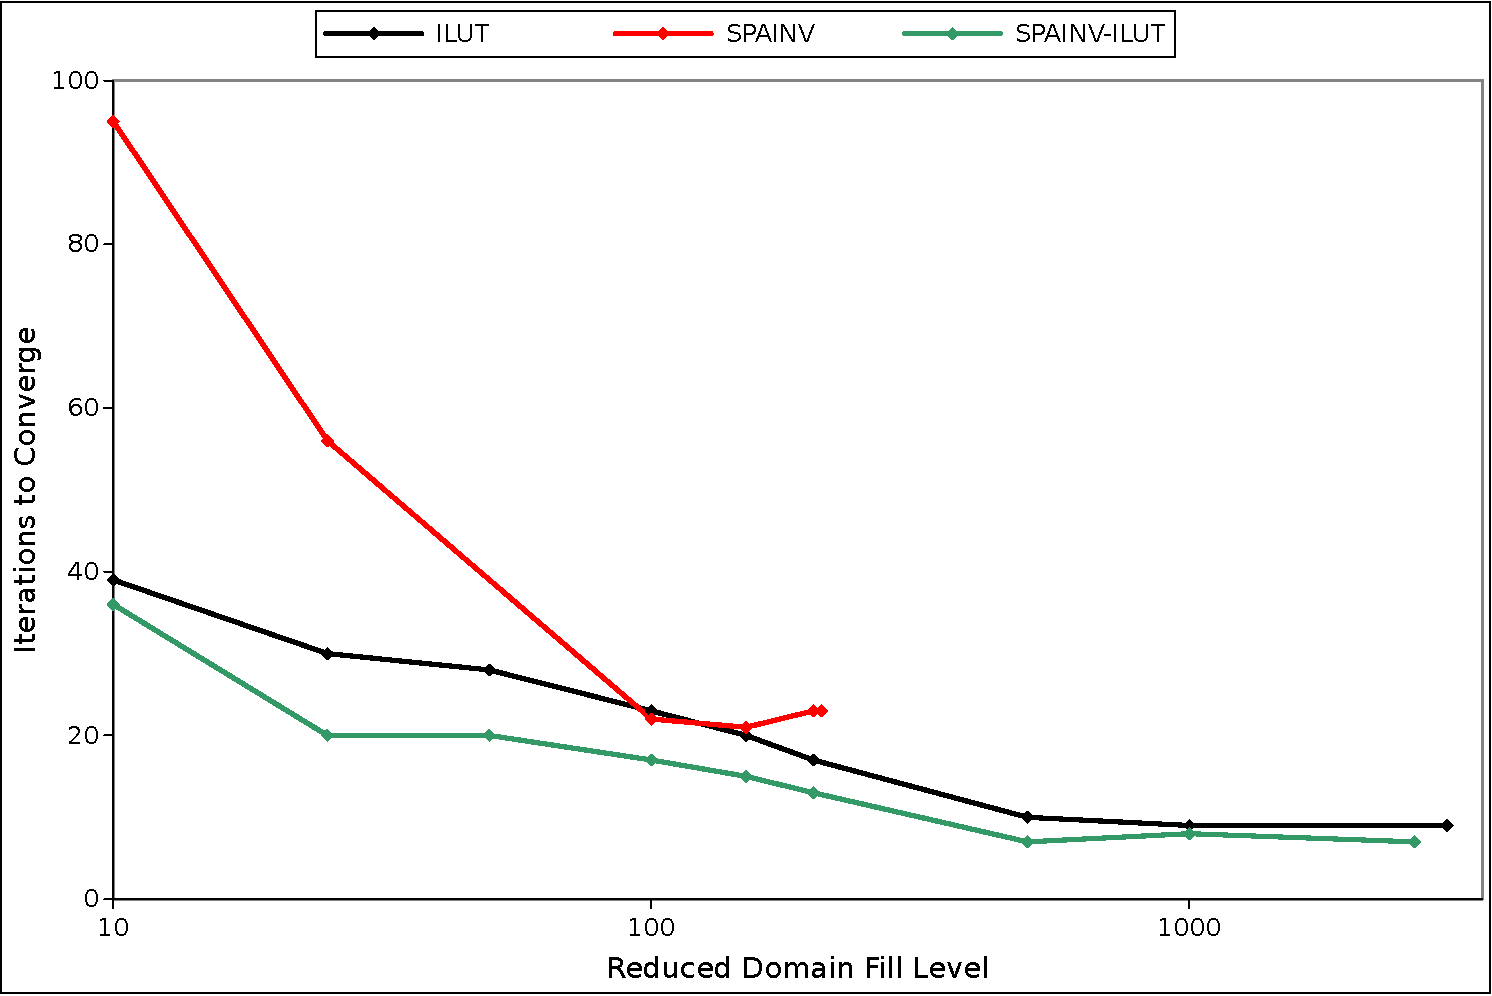
\includegraphics[width=4.25in]{rda_iterations.pdf}
  \end{center}
  \caption{\textbf{Number of MCSA iterations required to converge a
      single eigenvalue iteration for the fuel assembly problem with
      each preconditioning as a function of reduced domain
      approximation fill level.} \textit{The largest fill level for
      each preconditioning presented is that using the parameters that
      gave the best results without the approximation.}}
  \label{fig:rda_iterations}
\end{figure}

\begin{figure}[t!]
  \begin{center}
    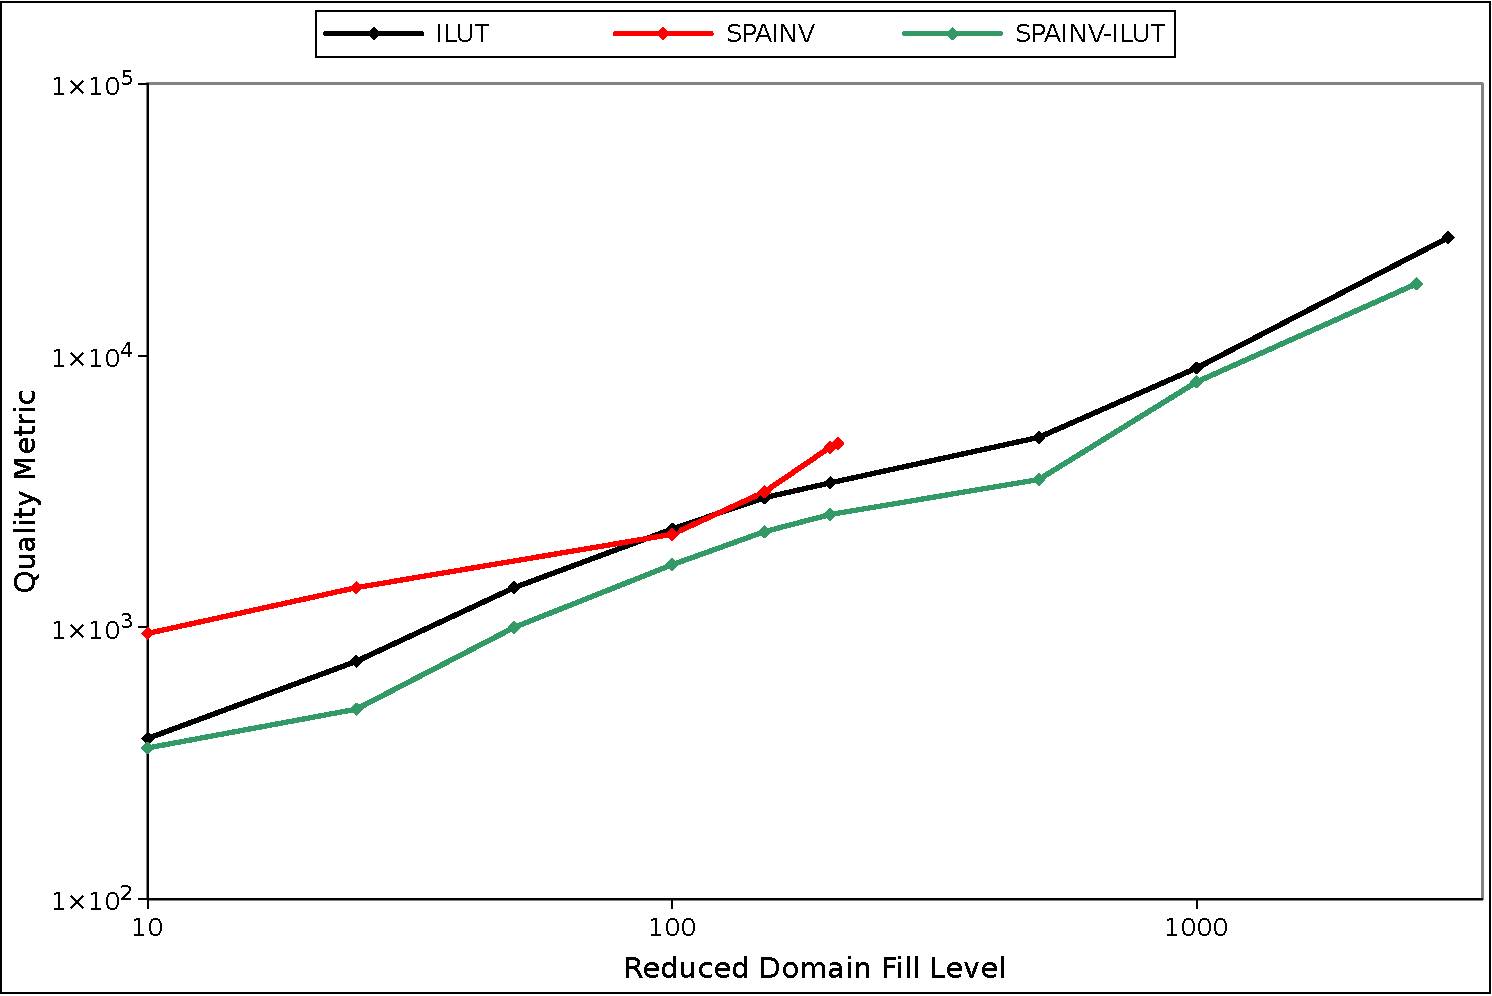
\includegraphics[width=4.25in]{rda_quality.pdf}
  \end{center}
  \caption{\textbf{Preconditioning quality metric for the fuel
      assembly problem given as a function of reduced domain
      approximation fill level.} \textit{The largest fill level for
      each preconditioning presented is that using the parameters that
      gave the best results without the approximation.}}
  \label{fig:rda_quality}
\end{figure}

\clearpage

\subsection{MCSA Relaxation Parameters}
\label{subsec:spn_mcsa_relaxation}
As another means of preconditioning (or variance reduction), the
Richardson iteration upon which the Neumann-Ulam method is built may
be implemented with a scalar relaxation parameter that can be adjusted
to improve convergence:
\begin{equation}
  \mathbf{x} = \mathbf{x} + \omega \mathbf{r}\:,
  \label{eq:richardson_relaxation}
\end{equation}
where $\omega$ is the relaxation parameter. This is very similar to
point Jacobi preconditioning where the system is being scaled on the
left by a constant value in all rows. Analogously, these relaxation
parameter techniques can be applied to Monte Carlo to improve
convergence as demonstrated by Dimov \cite{dimov_new_1998}. In this
case, building an iteration matrix from
Eq~(\ref{eq:richardson_relaxation}) gives:
\begin{equation}
  \mathbf{H} = \mathbf{I} - \omega \mathbf{A}\:,
  \label{eq:relaxed_iteration_matrix}
\end{equation}
with the probabilities and weights for the Monte Carlo procedure
appropriately scaled. By inspection, such a scaling is a simple form
of preconditioning on the left where all rows in the system are scaled
by the same scalar parameter. For MCSA, we can stage this scheme with
two separate relaxation parameters; one for the outer Richardson
iteration and one for the inner Monte Carlo solve:
\begin{subequations}
  \begin{gather}
    \ve{x}^{k+1/2} = \ve{x}^k + \omega_R \ve{r}^k\:,\\ \ve{r}^{k+1/2}
    = \ve{b} -
    \ve{A}\ve{x}^{k+1/2}\:,\\ \omega_N\ve{A}\delta\ve{x}^{k+1/2} =
    \omega_N\ve{r}^{k+1/2}\:,\\ \ve{x}^{k+1} = \ve{x}^{k+1/2} + \delta
    \ve{x}^{k+1/2}\:,\\ \ve{r}^{k+1} = \ve{b} - \ve{A}\ve{x}^{k+1}\:,
  \end{gather}
  \label{eq:mcsa_relaxed}
\end{subequations}
where $\omega_R$ is the Richardson iteration relaxation parameter and
$\omega_N$ is the Neumann-Ulam Monte Carlo solve relaxation parameter.

We apply these relaxation parameters to the fuel assembly problem
along with the reduced domain approximation as a means of studying
their effects. For each calculation presented, the number of
iterations required to converge reported was for a single eigenvalue
iteration.  Again, \sn{3}{4} histories are used at each MCSA iteration
to compute the Monte Carlo correction using the adjoint collision
estimator. A reduced domain fill level of 100 is used with a threshold
of \sn{1}{-10} to filter small values. ILUT preconditioning with a
drop tolerance of \sn{1}{-5} and fill level of 5 is used as
well. 

Figure~\ref{fig:relax_iters} gives the number of iterations required
to converge the fuel assembly problem for a 1-group SP1 discretization
using varying combinations of the relaxation parameters. First, both
parameters were fixed at the base case of 1 while the other parameter
was varied as shown in the left-hand side plots of
Figure~\ref{fig:relax_iters}. For the Richardson relaxation parameter,
using a value larger than 1 gave better iterative performance up to a
point, effectively providing a stronger extrapolation using the
residual at each iteration. For the Neumann relaxation parameter, a
value of less than 1 is observed to be ideal. Although initially
counter-intuitive, the fact that the correction computed by the Monte
Carlo solver has a stochastic error associated with it means that by
using a Neumann relaxation parameter less than 1, the correction and
its error are effectively dampened to improve iterative
performance. Considering the CPU time required to converge a single
eigenvalue iteration, similar results are also observed for the
relaxation parameters as given by Figure~\ref{fig:relax_time}. For the
base cases given by the plots on the left, it was found the a
Richardson relaxation parameter of 1.1 and a Neumann relaxation
parameter of 0.7 provided the fastest CPU time for convergence. Fixing
each parameter at these new values, the calculations were repeated as
shown for the plots on the right hand sides of both
Figures~\ref{fig:relax_iters} and \ref{fig:relax_time}. For each
repeated timing calculation, it was found that the same combination of
relaxation parameters found in the base cases performed the best
although they did not necessarily have the best iterative performance.

\begin{figure}[t!]
  \begin{center}
    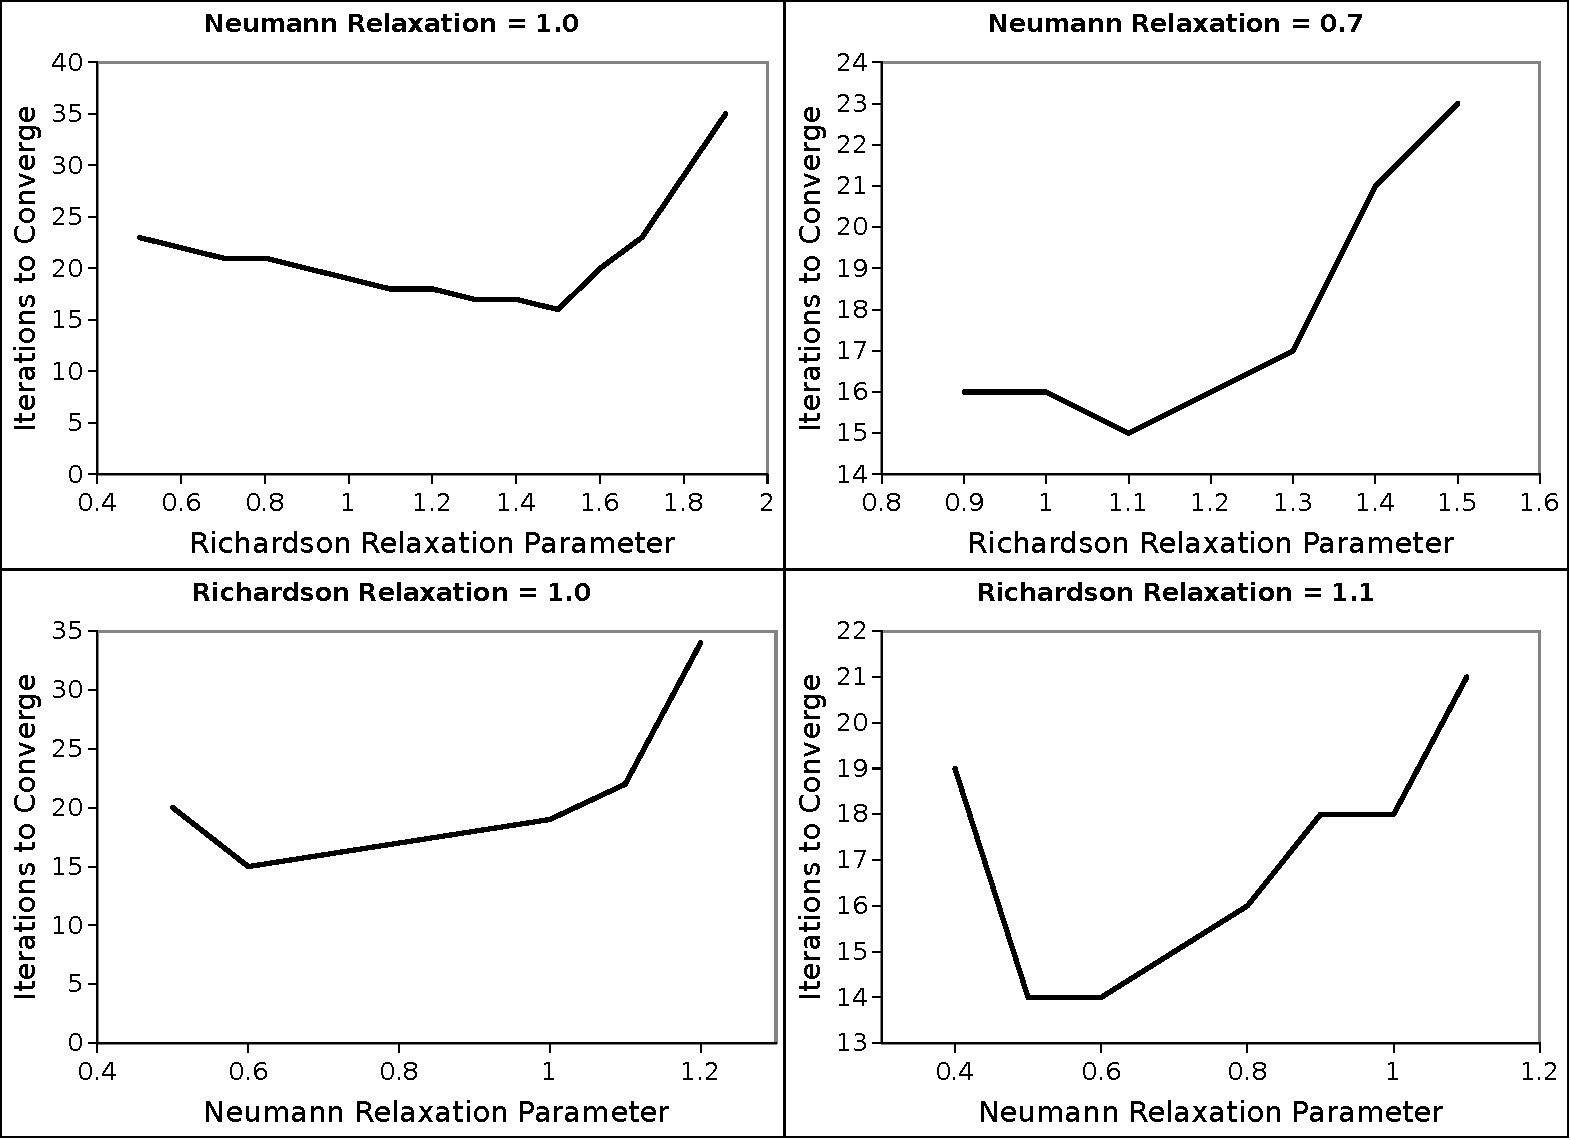
\includegraphics[width=6in]{relax_iters.pdf}
  \end{center}
  \caption{\textbf{Number of iterations to converge a single
      eigenvalue iteration of the fuel assembly problem as a function
      of the relaxation parameters.} \textit{Starting in upper left
      and moving counter-clockwise: Neumann relaxation parameter fixed
      at 1.0, Richardson relaxation parameter fixed at 1.0, Neumann
      relaxation parameter fixed at 0.7, Richardson relaxation
      parameter fixed at 1.1. For each calculation \sn{3}{4}
      stochastic histories were used to compute the MCSA correction at
      each iteration.}}
  \label{fig:relax_iters}
\end{figure}

\begin{figure}[t!]
  \begin{center}
    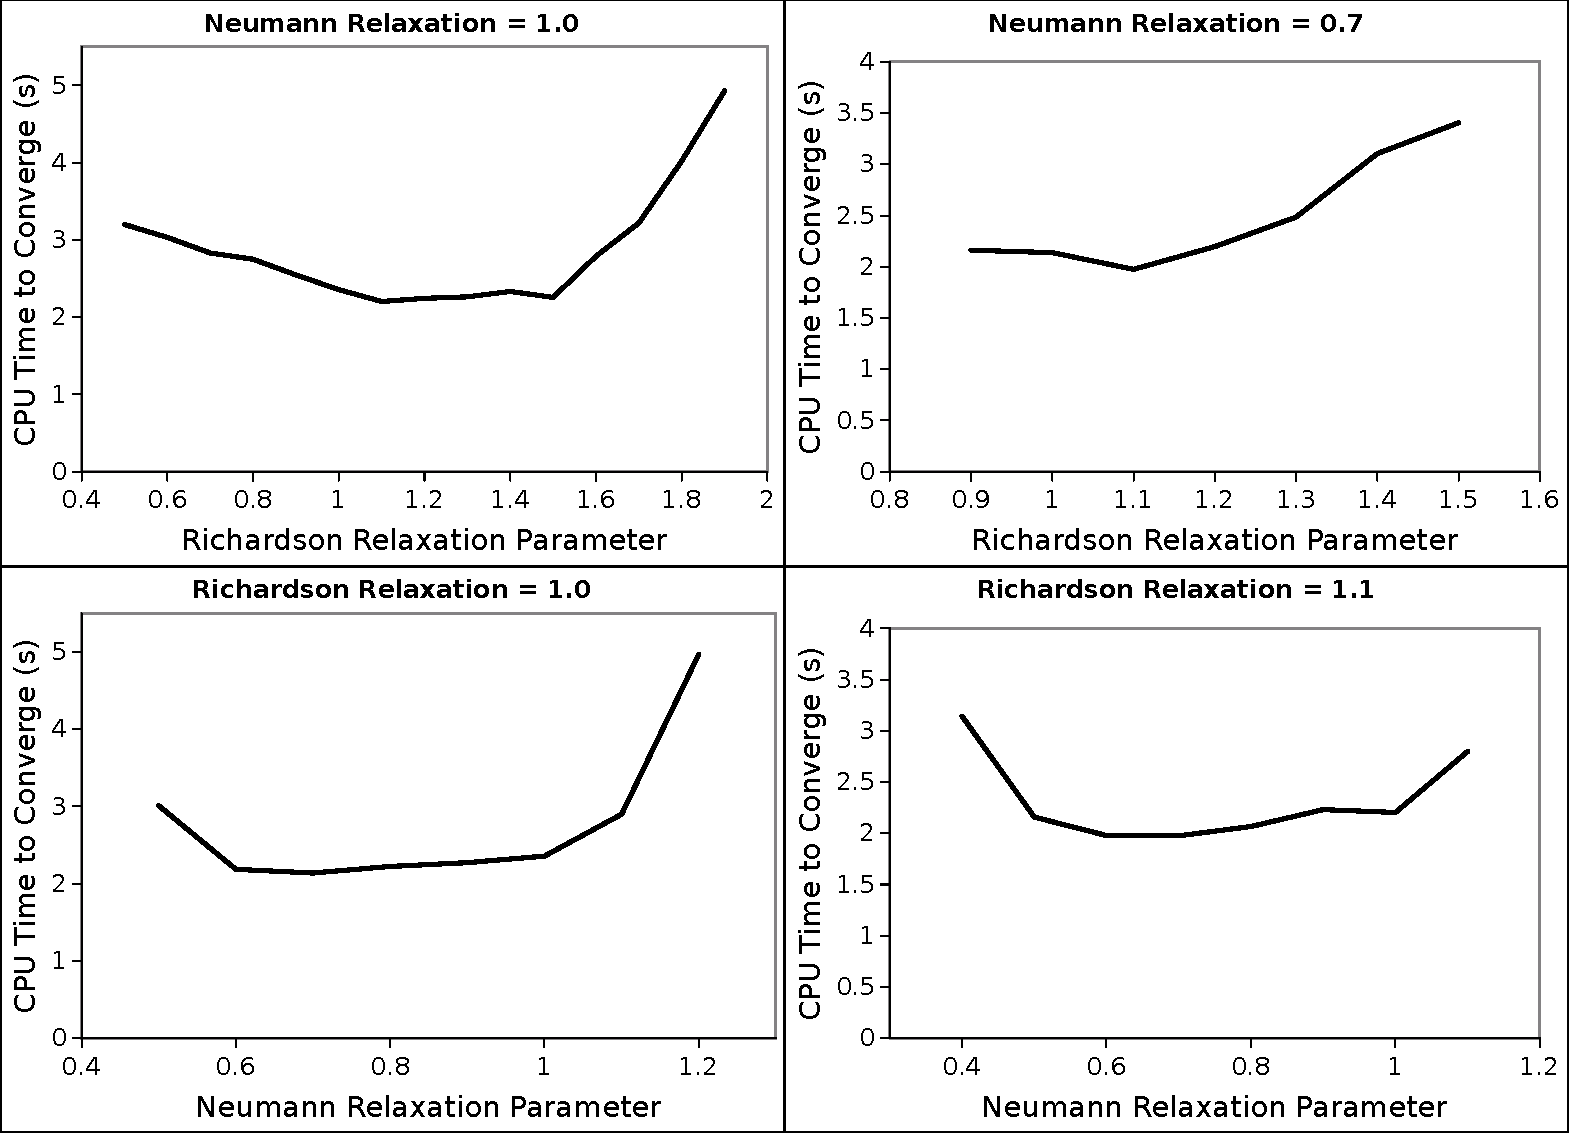
\includegraphics[width=6in]{relax_time.pdf}
  \end{center}
  \caption{\textbf{CPU time in seconds to converge a single eigenvalue
      iteration of the fuel assembly problem as a function of the
      relaxation parameters.} \textit{Starting in upper left and
      moving counter-clockwise: Neumann relaxation parameter fixed at
      1.0, Richardson relaxation parameter fixed at 1.0, Neumann
      relaxation parameter fixed at 0.7, Richardson relaxation
      parameter fixed at 1.1. For each calculation \sn{3}{4}
      stochastic histories were used to compute the MCSA correction at
      each iteration.}}
  \label{fig:relax_time}
\end{figure}

%%---------------------------------------------------------------------------%%
\section{Results}

Through the numerical studies presented in this chapter, we have
developed a set of preconditioning techniques that permit MCSA to be
used with the $SP_N$ form of the neutron transport equation and
applied to a difficult fuel assembly criticality problem. Along with
these preconditioning techniques, a set a varying MCSA parameters were
analyzed to find those that yielded the best performance for this
particular problem. In addition, several steps were taken to mitigate
the dense composite linear operators that arise when performing
explicit MCSA preconditioning in order to achieve convergence. Using
these results, we compare MCSA directly to conventional linear solvers
that would be typically used to solve the $SP_N$ form of the transport
equation as presented here. In particular, we will use a pair of
production Krylov solvers with which we will compare direct numerical
results in order to verify MCSA solutions in this section.

For the comparison calculations, all solvers will be preconditioned
with ILUT using a drop tolerance of \sn{1}{-5} and a fill level of
5. For GMRES, no restrictions were placed on the size of the subspace
and therefore no restarts occurred. When the collision estimator was
used with MCSA, \sn{2}{4} stochastic histories were used to compute
the correction for every energy group in the problem (\sn{4}{4} and
\sn{8}{4} histories total for the 2 and 4 group calculations
respectively) corresponding to approximately 1 stochastic history per
DOF. When the expected value estimator was used, \sn{5}{2} stochastic
histories used for each energy group (\sn{1}{3} and \sn{1.5}{3}
histories total for the 2 and 4 group calculations) giving
approximately 1 stochastic history for every 5 DOFs. The reduced
domain approximation was also applied in conjunction with the ILUT
preconditioning using a fill level of 100 and a threshold value of
\sn{1}{-10} to reduce the density of states in the Monte Carlo
problem. For relaxation parameters, all MCSA computations used a
Neumann relaxation parameter of 0.7 while a Richardson relaxation of
1.1 was used with the collision estimator and 1.0 with the expected
value estimator as determined by the previous analysis of the
relaxation parameters. Table~\ref{tab:spn_solver_defs} gives
definitions for the solvers used to generate the results in the
remainder of this section. For the energy group structures,
Table~\ref{tab:spn_group_structure} gives the lower bounds of each
group in eV (an implicit upper bound of \sn{2}{6} eV is assumed for
group 0).

To compare iterative performance, the number of linear solver
iterations required to converge each eigenvalue iteration was recorded
and then averaged over all eigenvalue iterations for each
solver. Figure~\ref{fig:spn_comparison_iterations} gives the average
number of linear solver iterations required to converge a single
eigenvalue iteration of the fuel assembly problem as a function of the
number of energy groups. In general, the iterative performance of all
the solvers tested is comparable with BiCGStab performing the best. We
expect this because not only are the multigroup $SP_N$ equations
elliptic and positive-definite, but they are also nearly symmetric and
therefore we expect the conjugate gradient-based methods to perform
well due to the structure of the projection scheme. It important to
note that the iterative performance of each solver is not a strong
function of the number of energy groups in the problem (and therefore
the problem size). Even more important, although BiCGStab produced the
best iterative results, MCSA did perform better than GMRES in many
cases with the Richardson iteration accelerated with Monte Carlo using
the collision estimator performing best.

For MCSA, we are linearly increasing the number of stochastic
histories used to compute the correction at each iteration as the
number of energy groups are increased and therefore the work performed
for the problem is of $O(N)$. It is also important to note the reduced
domain approximation parameters, particularly the fill level, were
fixed as the number of energy groups was increased. By fixing the fill
level, we are effectively fixing the amount of information contained
in the composite linear operator available for the Monte Carlo
problem. Limiting this information to 100 entries per row in the
preconditioned system did not appear to have a significant effect on
the iterative performance of the solver. For larger numbers of energy
groups (and therefore DOFs) this may be an issue and this number may
need to be increased to maintain iterative performance. Currently,
memory restrictions arising from the explicit preconditioning strategy
prevent larger energy groups to be analyzed using an appropriate
preconditioner for the fuel assembly problem.

\begin{figure}[t!]
  \begin{center}
    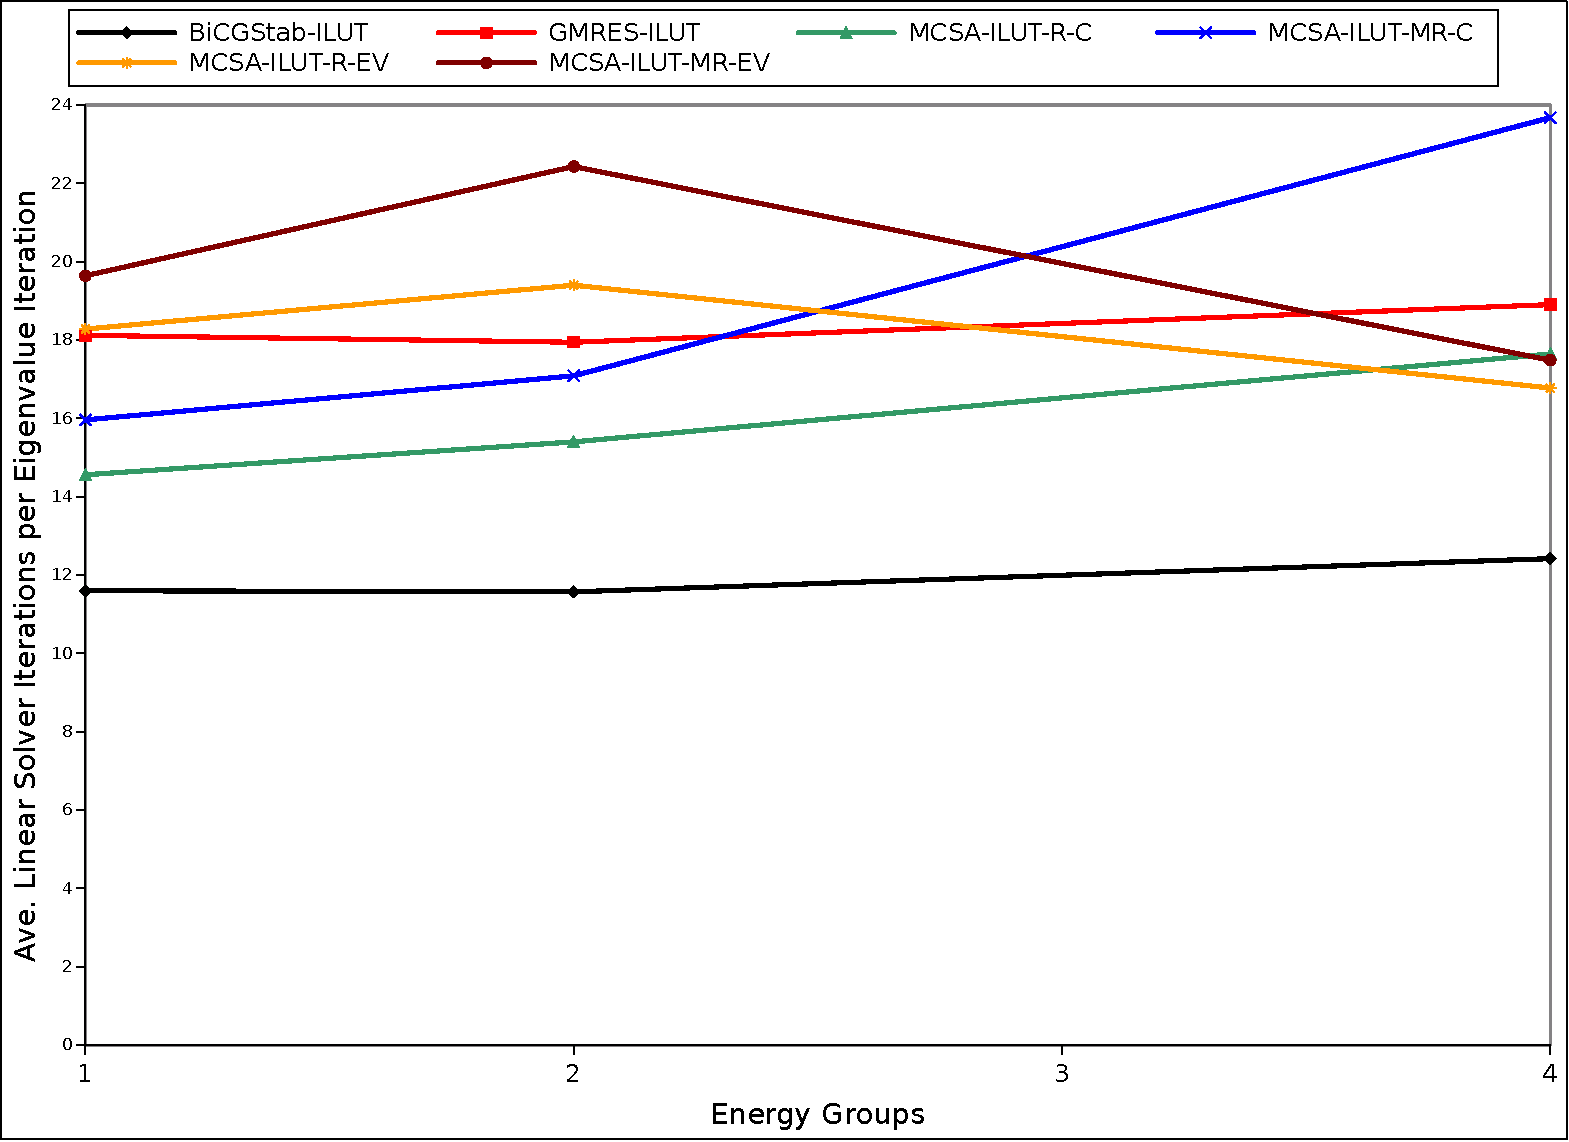
\includegraphics[width=5in]{solver_iters.pdf}
  \end{center}
  \caption{\textbf{Average number of iterations required to converge
      each eigenvalue iteration for the fuel assembly problem as a
      function of energy groups.}
    \textit{Table~\ref{tab:spn_solver_defs} gives the description for
      each solver type presented in the legend.}}
  \label{fig:spn_comparison_iterations}
\end{figure}

Although iterative performance for MCSA was comparable to that
observed for production Krylov implementations using exactly the same
preconditioning scheme, timing performance is not as competitive. For
this comparison, the amount of time to perform each linear solver
iteration in every eigenvalue iteration was recorded and then averaged
over all linear solver
iterations. Figure~\ref{fig:spn_comparison_time} gives the average CPU
time per linear solver iteration required to converge the fuel
assembly problem with all linear solver iterations over all eigenvalue
iterations used to compute the average. The production Krylov solver
implementations are approximately an order of magnitude faster than
the MCSA implementations presented here. We expect these results for
several reasons. First, even when the reduced domain approximation is
used there are $O(100)$ elements in each row of the system and each of
those elements must be processed during a transition in the Monte
Carlo random walk sequence. In addition, although the preconditioned
fixed point iterations used in the MCSA sequence do not use the
composite linear operator but rather a sequence of matrix vector
multiplies to achieve the same preconditioning effect, they do use the
explicitly extracted inverse of the preconditioning matrices which
themselves are dense, leading to exceedingly slow computation times
even in the fixed point iteration. For the production Krylov methods,
the ILUT preconditioners are applied to a vector with two triangular
solves, one for each triangular factor. Also, the original linear
operator has $O(10)$ elements in each row of the system, an order of
magnitude less than that used in the reduced domain composite
operator. Second, the implementation presented here has not been
optimized and it is likely that several components of the algorithm
can be implemented in a more desirable time complexity. The
production Krylov solvers presented here have enjoyed decades of
professional development and optimization. However, it is most
important to note here that the CPU timing data presented in
Figure~\ref{fig:spn_comparison_time} shows that all methods have the
same time complexity; their differences are merely the manifestation
of a large time constant due to the effects of the explicit
preconditioning scheme. For transport systems where this is not a
problem, the literature explicitly shows that MCSA can be competitive
with these production Krylov methods using CPU time as a measure
\cite{evans_monte_2012}.

\begin{figure}[t!]
  \begin{center}
    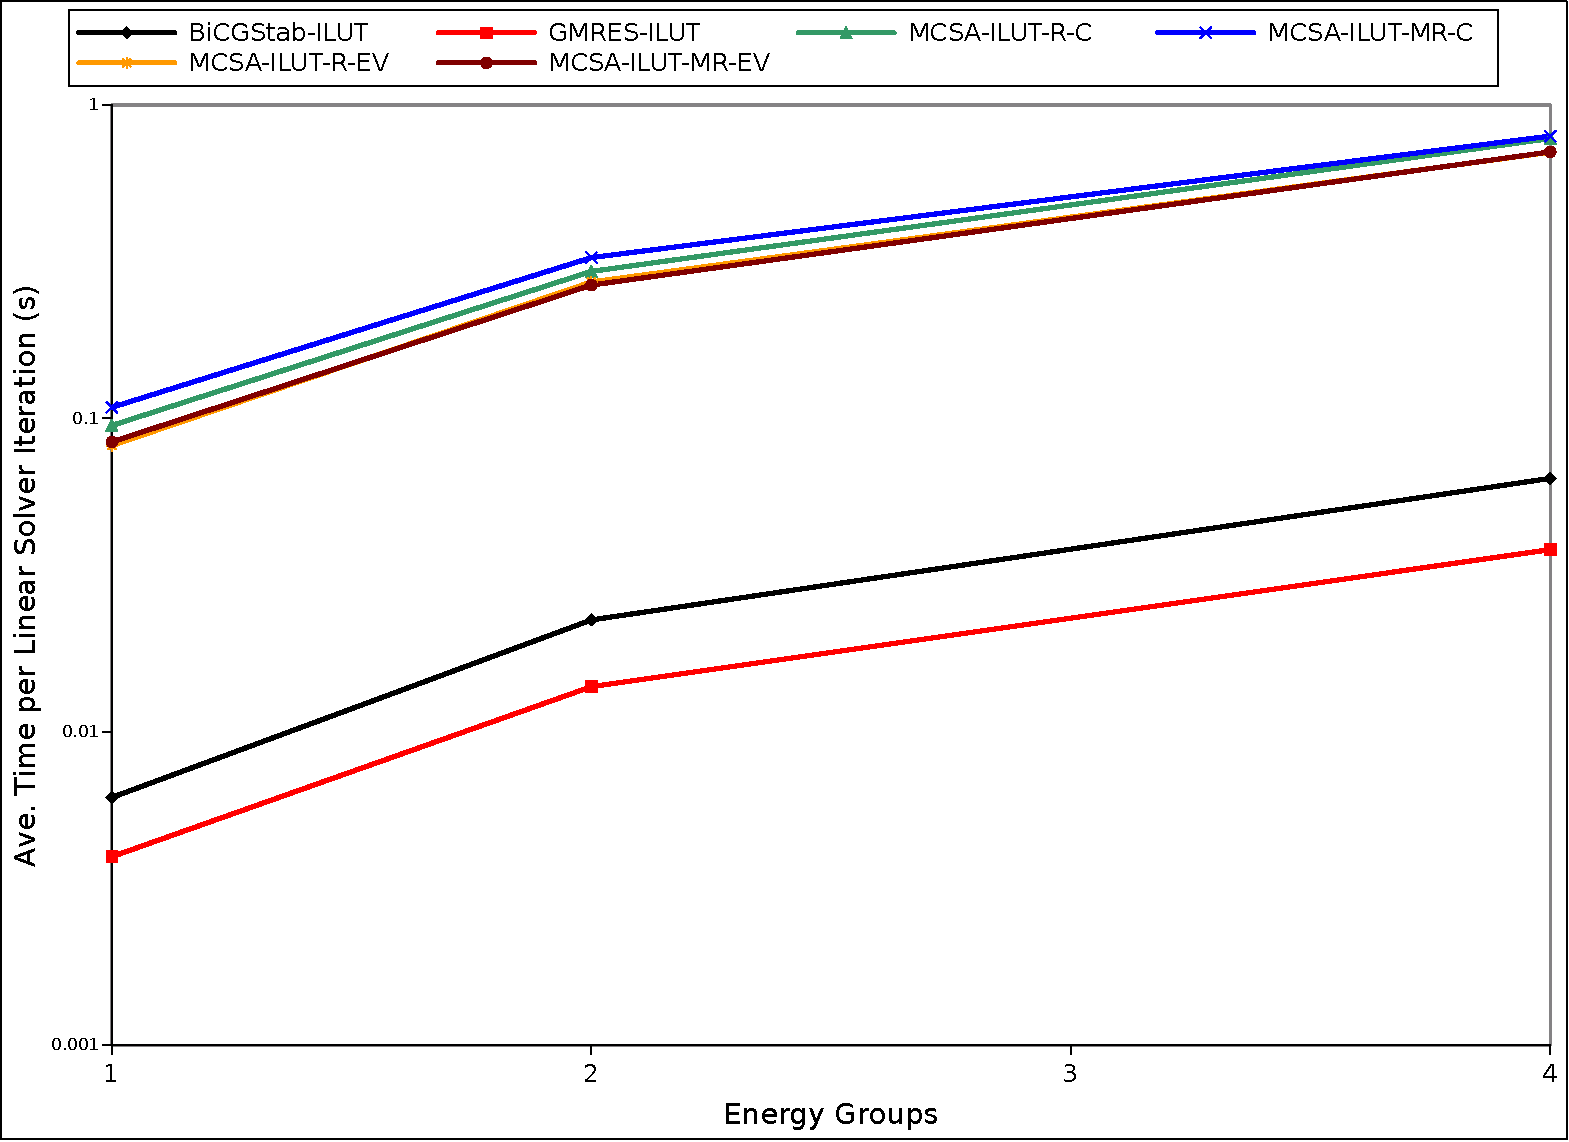
\includegraphics[width=5in]{solver_time.pdf}
  \end{center}
  \caption{\textbf{Average CPU time per linear solver iteration in
      seconds for the fuel assembly problem as a function of energy
      groups.}  \textit{All linear solver iterations over all
      eigenvalue iterations were used to compute the
      average. Table~\ref{tab:spn_solver_defs} gives the description
      for each solver type presented in the legend.}}
  \label{fig:spn_comparison_time}
\end{figure}

Finally, not considered in Figure~\ref{fig:spn_comparison_time} is the
time required to actually form the explicit inverse preconditioner
matrices and the composite operator through matrix-matrix
multiplication. The timing numbers reported were simply to perform the
MCSA iteration procedure with the composite operator already
formed. Figure~\ref{fig:spn_comparison_prec_time} additionally
presents the CPU times for MCSA convergence with the time to form the
inverse of the preconditioners and the composite linear operator
through matrix-matrix multiplication amortized over all iterations. As
is readily observed, including the costs of these operations increases
the MCSA computation time by another order of magnitude.

\begin{figure}[t!]
  \begin{center}
    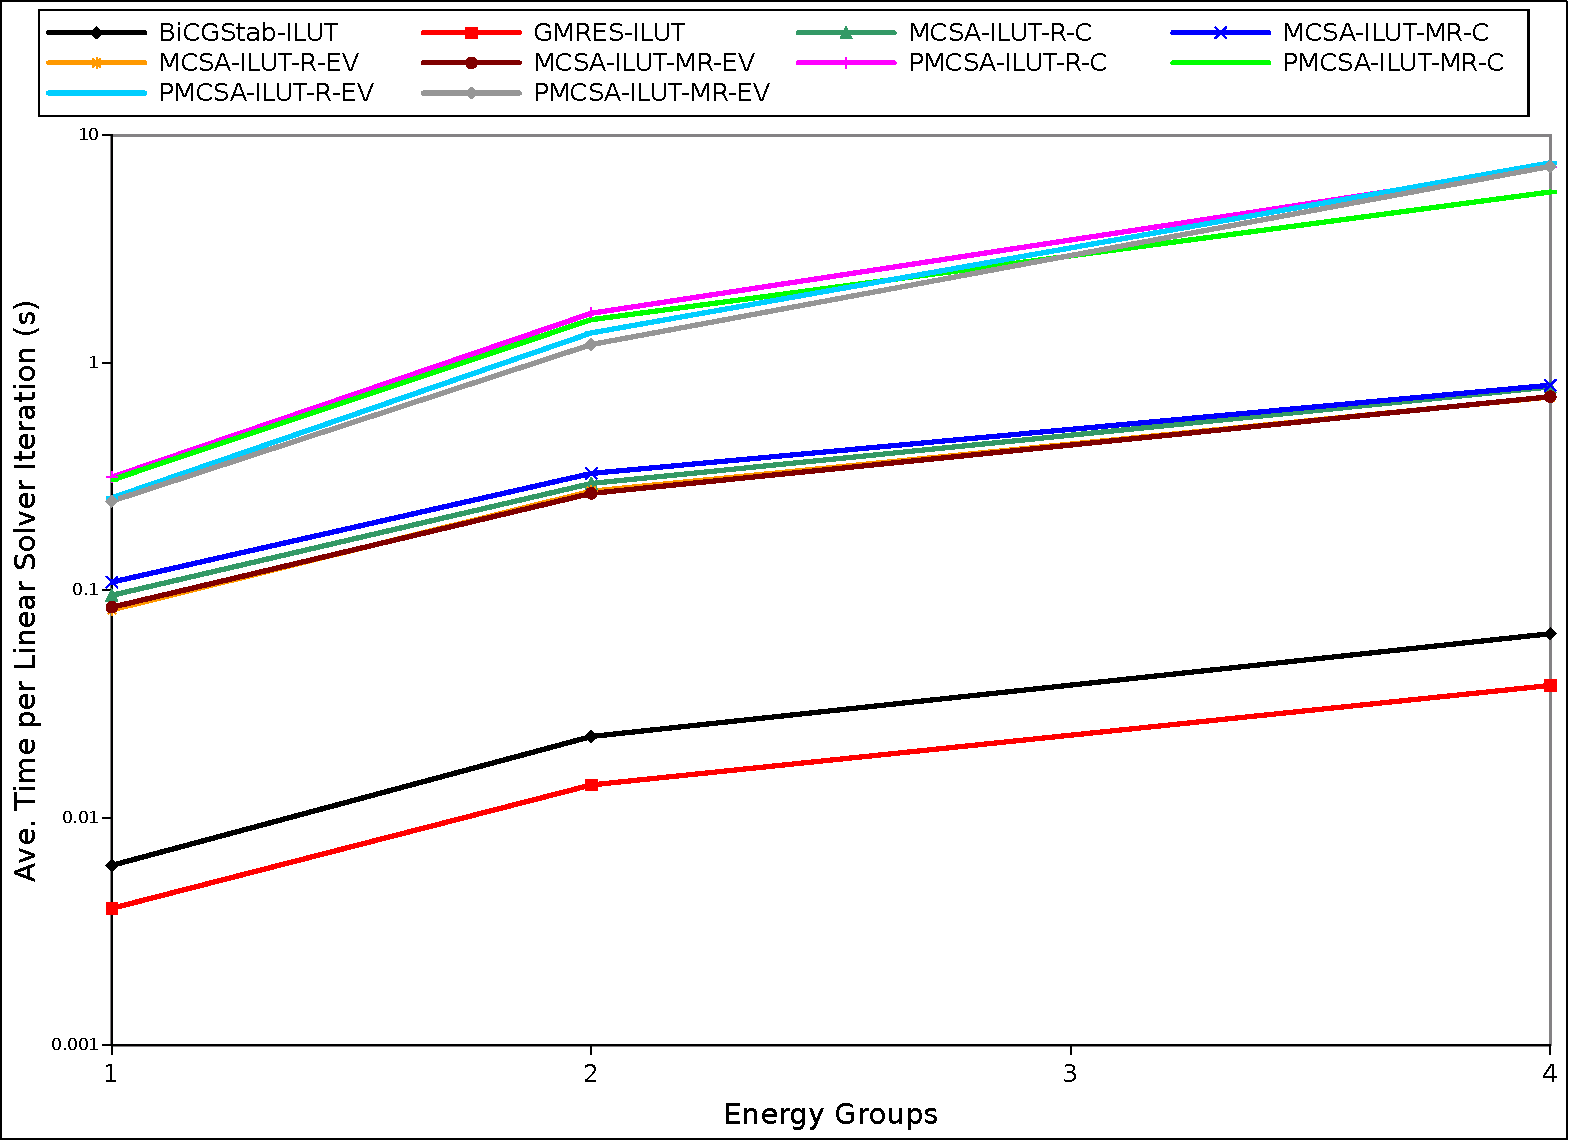
\includegraphics[width=5in]{solver_p_time.pdf}
  \end{center}
  \caption{\textbf{Average CPU time per iteration in seconds for the
      fuel assembly problem as a function of energy groups with
      preconditioning time included for the MCSA methods.}
    \textit{All linear solver iterations over all eigenvalue
      iterations were used to compute the
      average. Table~\ref{tab:spn_solver_defs} gives the description
      for each solver type presented in the legend. Data labeled
      starting with PMCSA is identical to those labeled with MCSA
      except that they additionally include the cost of generating the
      inverse of the preconditioners and composite linear operator.}}
  \label{fig:spn_comparison_prec_time}
\end{figure}

Based on the performance results in this section, MCSA shows promise
as a competitive and perhaps even superior method for solutions to the
neutron transport problem discretized with the $SP_N$
approximation. Not only are the correct answers produced when compared
to production linear solvers, but the iterative performance is
comparable to production Krylov methods with identical preconditioning
that would typically be used every-day calculations. From a CPU timing
perspective, the methods yield the same time complexity as a function
of the number of energy groups in the problem when compared to the
production Krylov methods. Here, a large time constant is generated
due to the explicit preconditioning strategy and the generation of
dense linear operators as a result. To improve these results and put
general MCSA schemes into a performance regime where they are
competitive with Krylov methods for neutron transport problems,
significant research will be required to improve upon the explicit
preconditioning scheme presented here.

%%---------------------------------------------------------------------------%%
\section{Conclusion}

%%---------------------------------------------------------------------------%%
\pagebreak
\bibliographystyle{ieeetr} \bibliography{references}
\end{document}


